\subsection{INVERSE LIMITS OF ALGEBRAIC STRUCTURES}

Let \((\mathbf{X}_{\alpha}, f_{\alpha\beta})\) be an inverse system of sets, and suppose that each \(X_{\alpha}\) is endowed with an internal law of composition, everywhere defined, and written multiplicatively. Suppose also that the \(f_{\alpha\beta}\) are homomorphisms with respect to these internal laws. Since

\[
f _ {\alpha \beta} (x _ {\beta}. y _ {\beta}) = f _ {\alpha \beta} (x _ {\beta}). f _ {\alpha \beta} (y _ {\beta})
\]

whenever \(\alpha \leqslant \beta\) and \(x_{\beta}\) and \(y_{\beta}\) belong to \(\mathbf{X}_{\beta}\) , it is clear that \(\mathbf{X} = \varprojlim \mathbf{X}_{\alpha}\) is a stable subset of the product \(\prod_{\alpha} \mathbf{X}_{\alpha}\) , with respect to the internal law \((x_{\alpha}) \cdot (y_{\alpha}) = (x_{\alpha} \cdot y_{\alpha})\) . Let \((\Lambda_{\alpha}, \varphi_{\alpha\beta})\) be another inverse system of sets, indexed by I, and suppose that each \(\mathbf{X}_{\alpha}\) carries an external law of composition, everywhere defined, written multiplicatively and having \(\Lambda_{\alpha}\) as a set of operators, such that whenever \(\alpha \leqslant \beta\) we have

\[
f _ {\alpha \beta} (\lambda_ {\beta}. x _ {\beta}) = \varphi_ {\alpha \beta} (\lambda_ {\beta}). f _ {\alpha \beta} (x _ {\beta})
\]

for \(\lambda_{\beta} \in \Lambda_{\beta}\) and \(x_{\beta} \in X_{\beta}\) . Then we can define an external law on \(\prod_{\alpha} X_{\alpha}\) , having \(\prod_{\alpha} \Lambda_{\alpha}\) as a set of operators, by defining \((\lambda_{\alpha}) \cdot (x_{\alpha}) = (\lambda_{\alpha} \cdot x_{\alpha})\) ; restricting the set of operators to \(\Lambda = \varprojlim \Lambda_{\alpha}\) , we have an external law on \(\prod_{\alpha} X_{\alpha}\) with respect to which \(X\) is again a stable subset. The internal

(resp. external) law thus defined on X is said to be the inverse limit of the internal (resp. external) laws of the \(X_{\alpha}\) . In the case of external laws, it may happen that all the \(\Lambda_{\alpha}\) are identical with the same set \(\Lambda_{0}\) and that all the \(\varphi_{\alpha \beta}\) are identity mappings; then, since I is a directed set, \(\Lambda\) can be identified with \(\Lambda_0\) .

It is immediately verified that the usual properties of associativity, commutativity, existence of an identity element for an internal law (provided that the \(f_{\alpha\beta}\) map identity element to identity element), distributivity of an external law with respect to an internal law, etc., are preserved under passage to the inverse limit.

Let \(\Sigma\) be a species of algebraic structure and let \(\Sigma_0\) be the impoverished structure corresponding to \(\Sigma\) . Whenever we speak of an inverse system of sets \((\mathbf{X}_{\alpha}, f_{\alpha\beta})\) endowed with structures of species \(\Sigma\) , we shall always suppose that the \(f_{\alpha\beta}\) are homomorphisms for these structures. If we endow \(\mathbf{X} = \varprojlim \mathbf{X}_{\alpha}\) with the internal and external laws which are the respective inverse limits of the internal and external laws of the \(\mathbf{X}_{\alpha}\) , then \(\mathbf{X}\) carries an algebraic structure of species \(\Sigma_0\) . Naturally it remains to be seen in each particular case whether or not this structure is of species \(\Sigma\) .

For example, if \((\mathbf{G}_{\alpha}, f_{\alpha\beta})\) is an inverse system of groups (resp. rings), then \(\varprojlim G_{\alpha}\) is a subgroup (resp. subring) of \(\prod_{\alpha} G_{\alpha}\) , and is called the inverse limit of the system \((\mathbf{G}_{\alpha}, f_{\alpha\beta})\) of groups (resp. rings).

Let \((\mathbf{X}_{\alpha}, g_{\alpha \beta})\) be an inverse system of sets and let \((\mathbf{G}_{\alpha}, f_{\alpha \beta})\) be an inverse system of groups; suppose that each \(\mathbf{X}_{\alpha}\) has \(\mathbf{G}_{\alpha}\) as a group of operators and that whenever \(\alpha \leqslant \beta\) we have

\[
g _ {\alpha \beta} (s _ {\beta}. x _ {\beta}) = f _ {\alpha \beta} (s _ {\beta}). g _ {\alpha \beta} (x _ {\beta})\tag{1}
\]

for \(x_{\beta} \in X_{\beta}\) and \(s_{\beta} \in G_{\beta}\) . Then \(X = \varprojlim X_{\alpha}\) has \(G = \varprojlim G_{\alpha}\) as group of operators. It follows from (1) that, if \(\alpha \leqslant \beta\) , the mappings \(f_{\alpha \beta}\) and \(g_{\alpha \beta}\) are compatible (§ 2, no. 4) and hence define a mapping \(\varphi_{\alpha \beta}: X_{\beta}/G_{\beta} \to X_{\alpha}/G_{\alpha}\) of the quotient sets, such that \((X_{\alpha}/G_{\alpha}, \varphi_{\alpha \beta})\) is an inverse system. Moreover, if \(f_{\alpha}: G \to G_{\alpha}\) and \(g_{\alpha}: X \to X_{\alpha}\) are the canonical mappings, then \(f_{\alpha}\) and \(g_{\alpha}\) are compatible and consequently define a mapping \(h_{\alpha}: X/G \to X_{\alpha}/G_{\alpha}\) of the quotient sets; it is clear that the \(h_{\alpha}\) form an inverse system of mappings, whose inverse limit is therefore a mapping \(h: X/G \to \varprojlim X_{\alpha}/G_{\alpha}\) , which is not necessarily either injective or surjective (Exercise 1).

Again, let \((\mathbf{A}_{\alpha}, \varphi_{\alpha\beta})\) be an inverse system of rings and let \((\mathbf{M}_{\alpha}, f_{\alpha\beta})\) be an inverse system of commutative groups; and suppose that each \(M_{\alpha}\) carries a left \(A_{\alpha}\) -module structure in such a way that whenever \(\alpha \leqslant \beta\) we have

\[
f _ {\alpha \beta} (\lambda_ {\beta}. x _ {\beta}) = \varphi_ {\alpha \beta} (\lambda_ {\beta}). f _ {\alpha \beta} (x _ {\beta})\tag{2}
\]

for \(x_{\beta} \in M_{\beta}\) and \(\lambda_{\beta} \in A_{\beta}\) ; then \(\varprojlim M_{\alpha}\) has a structure of a left module over \(\varprojlim A_{\alpha}\) . If we suppose in addition that, for each \(\alpha\) , \(A_{\alpha}\) is commutative and that each \(M_{\alpha}\) has an \(A_{\alpha}\) -algebra structure, and finally that \((\mathbf{M}_{\alpha}, f_{\alpha\beta})\) is an inverse system of rings, then \(\varprojlim M_{\alpha}\) has a structure of an algebra over \(\varprojlim A_{\alpha}\) .

Let \((\mathbf{G}_{\alpha}, f_{\alpha \beta})\) be an inverse system of groups, and for each \(\alpha\) let \(\mathbf{H}_{\alpha}\) be a subgroup of \(\mathbf{G}_{\alpha}\) . If \(f_{\alpha \beta}(\mathbf{H}_{\beta}) \subset \mathbf{H}_{\alpha}\) whenever \(\alpha \leqslant \beta\) , then the inverse system of subsets \(\mathbf{H}_{\alpha}\) of \(\mathbf{G}_{\alpha}\) is an inverse system of groups with respect to the restrictions of the \(f_{\alpha \beta}\) , and \(\mathbf{H} = \varprojlim \mathbf{H}_{\alpha}\) is a subgroup of \(\mathbf{G} = \varprojlim \mathbf{G}_{\alpha}\) . If each \(\mathbf{H}_{\alpha}\) is a normal subgroup of \(\mathbf{G}_{\alpha}\) , then \(\mathbf{H}\) is a normal subgroup of \(\mathbf{G}\) . If \((\mathbf{G}_{\alpha}', f_{\alpha \beta}')\) is another inverse system of groups and, for each \(\alpha, u_{\alpha}: \mathbf{G}_{\alpha} \to \mathbf{G}_{\alpha}'\) is a homomorphism such that the \(u_{\alpha}\) form an inverse system of mappings, then, if \(\mathbf{H}_{\alpha}\) is the kernel of \(u_{\alpha}\) , we have \(f_{\alpha \beta}(\mathbf{H}_{\beta}) \subset \mathbf{H}_{\alpha}\) whenever \(\alpha \leqslant \beta\) ; \(u = \varprojlim u_{\alpha}\) is a homomorphism of \(\mathbf{G}\) into \(\mathbf{G}' = \varprojlim \mathbf{G}_{\alpha}'\) , and \(\mathbf{H} = \varprojlim \mathbf{H}_{\alpha}\) is the kernel of \(u\) . If we put \(\mathbf{K}_{\alpha} = u_{\alpha}(\mathbf{G}_{\alpha})\) , then we have \(f_{\alpha\beta}'(\mathbf{K}_{\beta}) \subset \mathbf{K}_{\alpha}\) whenever \(\alpha \leqslant \beta\) , so that the \(\mathbf{K}_{\alpha}\) form an inverse system of subgroups of the \(\mathbf{G}_{\alpha}'\) ; but \(\mathbf{K} = \varprojlim \mathbf{K}_{\alpha}\) is not necessarily the image of \(\mathbf{G}\) under \(u\) {[}Exercise 1 c){]}.

\pandocbounded{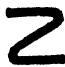
\includegraphics[keepaspectratio]{images/part002_764ec905.jpg}}

We obtain analogous results by replacing ``group'' by ``ring'', ``subgroup'' by ``ideal'' (left or right); we leave to the reader the task of stating the analogous results for modules and algebras.

\subsection{INVERSE LIMITS OF TOPOLOGICAL GROUPS AND SPACES WITH OPERATORS}

We shall say that an inverse system \((\mathbf{G}_{\alpha}, f_{\alpha\beta})\) is an inverse system of topological groups if the \(G_{\alpha}\) are topological groups and the \(f_{\alpha\beta}\) are continuous homomorphisms. Then \(G = \varprojlim G_{\alpha}\) is a subgroup of the product group \(\prod_{\alpha} G_{\alpha}\) ; if we endow G with the topological group structure induced by that of \(\prod_{\alpha} G_{\alpha}\) , then the topological group so obtained is called the inverse limit of the inverse system of topological groups \((\mathbf{G}_{\alpha}, f_{\alpha\beta})\) . If the \(G_{\alpha}\) are Hausdorff (resp. Hausdorff and complete) then G is Hausdorff and closed in \(\prod_{\alpha} G_{\alpha}\) (resp. Hausdorff and complete) (Chapter I, § 8, no. 2, Proposition 7, Corollary 2 and Chapter II, § 3, no. 5, Corollary to Proposition 10).

If \((\mathbf{G}_{\alpha}^{\prime}, f_{\alpha\beta}^{\prime})\) is another inverse system of topological groups and if, for each \(\alpha\) , \(u_{\alpha}: G_{\alpha} \to G_{\alpha}^{\prime}\) is a continuous homomorphism such that the \(u_{\alpha}\) form an inverse system of mappings, then \(u = \varprojlim u_{\alpha}\) is a continuous homomorphism of G into \(G^{\prime} = \varprojlim G_{\alpha}^{\prime}\) (Chapter I, § 4, no. 4). The same results are valid when ``topological group'' is replaced by ``topological ring''; we leave to the reader the task of stating the analogous results for topological modules (§ 6, no. 6).

Let \((\mathbf{X}_{\alpha}, g_{\alpha \beta})\) be an inverse system of topological spaces, and let \((\mathbf{G}_{\alpha}, f_{\alpha \beta})\) be an inverse system of topological groups. Suppose that each \(\mathbf{G}_{\alpha}\) operates continuously on \(\mathbf{X}_{\alpha}\) (§ 2, no. 4) and that the relations (1) hold for all \(x_{\beta} \in \mathbf{X}_{\beta}\) , \(s_{\beta} \in \mathbf{G}_{\beta}\) and \(\alpha \leqslant \beta\) . We have seen (no. 1) that \(\mathbf{X} = \varprojlim \mathbf{X}_{\alpha}\) has \(\mathbf{G} = \varprojlim \mathbf{G}_{\alpha}\) as group of operators; furthermore, \(\mathbf{G}\) operates continuously on \(\mathbf{X}\) . For if \(g_{\alpha}\) (resp. \(f_{\alpha}\) ) is the canonical mapping \(\mathbf{X} \to \mathbf{X}_{\alpha}\) (resp. \(\mathbf{G} \to \mathbf{G}_{\alpha}\) ), then by definition

\[
g _ {\alpha} (s, x) = f _ {\alpha} (s). g _ {\alpha} (x)
\]

and therefore the mappings \((s.x) \to g_{\alpha}(s.x)\) are continuous on \(\mathbf{X} \times \mathbf{G}\) , which shows the continuity of \((s, x) \to (s.x)\) (Chapter I, § 4, no. 4).

The mapping \(h_{\alpha}: \mathbf{X} / \mathbf{G} \to \mathbf{X}_{\alpha} / \mathbf{G}_{\alpha}\) induced by \(f_{\alpha}\) and \(g_{\alpha}\) is therefore continuous (§ 2, no. 4), and so is the mapping \(h: \mathbf{X} / \mathbf{G} \to \varprojlim \mathbf{X}_{\alpha} / \mathbf{G}_{\alpha}\) defined by the \(h_{\alpha}\) (Chapter I, § 2, no. 3, Proposition 4).

PROPOSITION 1. Suppose that the \(\mathbf{X}_{\alpha}\) and the \(\mathbf{G}_{\alpha}\) satisfy the above hypotheses. a) If the stabilizer of each point of \(\mathbf{X}_{\alpha}\) is a compact subgroup of \(\mathbf{G}_{\alpha}\) for each \(\alpha \in \mathbf{I}\) , then the stabilizer of each point \(x = (x_{\alpha})\) of \(\mathbf{X}\) is a compact subgroup of \(\mathbf{G}\) ; the orbit of \(x\) (with respect to \(\mathbf{G}\) ) is canonically homeomorphic to the inverse limit of the orbits of the \(x_{\alpha}\) (with respect to \(\mathbf{G}_{\alpha}\) ); and the canonical mapping \(h: \mathbf{X} / \mathbf{G} \to \varprojlim \mathbf{X}_{\alpha} / \mathbf{G}_{\alpha}\) is injective.

\begin{enumerate}
\def\labelenumi{\alph{enumi})}
\setcounter{enumi}{1}
\tightlist
\item
  If, for each \(\alpha \in \mathbf{I}\) , every orbit of a point of \(\mathbf{X}_{\alpha}\) (with respect to \(\mathbf{G}_{\alpha}\) ) is compact, then every orbit of a point of \(\mathbf{X}\) (with respect to \(\mathbf{G}\) ) is relatively compact, and \(h\) is surjective. If also \(h\) is bijective, then every orbit of a point of \(\mathbf{X}\) is compact.
\end{enumerate}

Let \(x = (x_{\alpha}) \in \mathbf{X}\) , and for each \(\alpha \in \mathbf{I}\) let \(\mathbf{X}_{\alpha}' = \mathbf{G}_{\alpha}.x_{\alpha}\) be the orbit of \(x_{\alpha}\) . If \(\alpha \leqslant \beta\) , it follows from (1) and the relation \(g_{\alpha\beta}(x_{\beta}) = x_{\alpha}\) that \(g_{\alpha\beta}(\mathbf{X}_{\beta}') \subset \mathbf{X}_{\alpha}',\) and hence that \((\mathbf{X}_{\alpha}')\) is an inverse system of subsets of the \(\mathbf{X}_{\alpha}\) . For each \(\alpha \in \mathbf{I}\) let \(u_{\alpha}: \mathbf{G}_{\alpha} \to \mathbf{X}_{\alpha}'\) be the continuous mapping \(s_{\alpha} \to s_{\alpha}.x_{\alpha}\) ; the \(u_{\alpha}\) form an inverse system of mappings, and \(u = \varprojlim u_{\alpha}\) is the continuous mapping \(s \to s.x\) of \(G\) into the subspace \(X' = \varprojlim X_{\alpha}'\) of \(X\) . The hypothesis of a) implies that \(\overline{u}_{\alpha}^{-1}(y_{\alpha})\) is compact for each \(y_{\alpha} \in X_{\alpha}'\) . Since also \(u_{\alpha}\) is surjective, the conditions of Chapter I, § 9, no. 6, Proposition 8, Corollary 2 are satisfied, and the first two assertions of a) are therefore established. Hence, if \(x = (x_{\alpha})\) and \(y = (y_{\alpha})\) are such that \(x_{\alpha}\) and \(y_{\alpha}\) belong to the same orbit with respect to \(G_{\alpha}\) for each \(\alpha \in I\) , then \(x\) and \(y\) belong to the same orbit with respect to \(G\) , and therefore \(h\) is injective.

Likewise, the hypothesis of b) implies that the inverse system of canonical mappings \(v_{\alpha}: \mathbf{X}_{\alpha} \to \mathbf{X}_{\alpha}/\mathbf{G}_{\alpha}\) satisfies the conditions of Chapter I, § 9, no. 6, Proposition 8, Corollary 2, and therefore its inverse limit \(v = \varprojlim v_{\alpha}: \mathbf{X} \to \varprojlim \mathbf{X}_{\alpha}/\mathbf{G}_{\alpha}\) is surjective, and the inverse image under \(v\) of every point of \(\varprojlim X_{\alpha}/G_{\alpha}\) is compact. Since \(v\) factorizes into

\[
\mathrm{X} \xrightarrow {\psi} \mathrm{X} / \mathrm{G} \xrightarrow {h} \varprojlim \mathrm{X} _ {\alpha} / \mathrm{G} _ {\alpha},
\]

where \(\psi\) is the canonical mapping, the assertions of b) follow.

COROLLARY 1. If the \(\mathbf{G}_{\alpha}\) are compact and the \(\mathbf{X}_{\alpha}\) Hausdorff, then the conclusions of a) and b) are valid.

For the hypotheses of a) and b) are satisfied, since every closed subgroup of \(G_{\alpha}\) is compact and \(u_{\alpha}: s_{\alpha} \to s_{\alpha}.x_{\alpha}\) is a continuous mapping of a compact space into a Hausdorff space.

COROLLARY 2. If, for each \(\alpha \in I\) , the group \(G_{\alpha}\) operates transitively on the space \(X_{\alpha}\) , and if the stabilizer of each point of \(X_{\alpha}\) is a compact subgroup of \(G_{\alpha}\) , then \(G\) operates transitively on \(X\) and the stabilizer of each point of \(X\) is a compact subgroup of \(G\) .

For hypothesis \(a)\) is satisfied, and \(\mathbf{X}_{\alpha}^{\prime} = \mathbf{X}_{\alpha}\) for each \(\alpha\) .

COROLLARY 3. Suppose that the \(\mathbf{G}_{\alpha}\) are Hausdorff. For each \(\alpha \in \mathbf{I}\) , let \(\mathbf{K}_{\alpha}\) be a compact subgroup of \(\mathbf{G}_{\alpha}\) , such that \(f_{\alpha \beta}(\mathbf{K}_{\beta}) \subset \mathbf{K}_{\alpha}\) whenever \(\alpha \leqslant \beta\) . Then, if \(\mathbf{K} = \varprojlim \mathbf{K}_{\alpha}\) , the canonical mapping \(h\) of the homogeneous space \(\mathbf{G} / \mathbf{K}\) into \(\varprojlim \mathbf{G}_{\alpha} / \mathbf{K}_{\alpha}\) is a homeomorphism.

The fact that \(h\) is bijective follows from Corollary 1, applied by replacing \(\mathbf{X}_{\alpha}\) by \(\mathbf{G}_{\alpha}\) , and \(\mathbf{G}_{\alpha}\) by \(\mathbf{K}_{\alpha}\) operating by right translations (§ 2, no. 5). Let \(\varphi\) be the canonical mapping \(\mathbf{G} \to \mathbf{G} / \mathbf{K}\) , and for each \(\alpha\) let \(f_{\alpha}\) be the canonical mapping \(\mathbf{G} \to \mathbf{G}_{\alpha}\) . If, for each \(\alpha, \mathbf{V}_{\alpha}\) runs through a fundamental system of open neighbourhoods of the identity element \(e_{\alpha}\) of \(\mathbf{G}_{\alpha}\) , then the sets \(\mathbf{V} = \overline{f}_{\alpha}^{-1}(\mathbf{V}_{\alpha}) (\alpha \text{ and } \mathbf{V}_{\alpha} \text{ variable})\) form a fundamental system of neighbourhoods of the identity element \(e\) in \(\mathbf{G}\) (Chapter I, § 4, no. 4, Proposition 9), and the sets \(\varphi(\mathbf{V}.K)\) form a fundamental system of neighbourhoods of \(\varphi(e)\) in \(G/K\) . We have to show that the image of \(\varphi(V.K)\) under \(h\) contains a neighbourhood of \(h(\varphi(e))\) , that is that there exists \(\beta \geqslant \alpha\) and a neighbourhood \(W_{\beta}\) of \(e_{\beta}\) in \(G_{\beta}\) such that \(\overline{f}_{\beta}^{-1}(W_{\beta}.K_{\beta}) \subset V.K\) . Now, the relation \(x \in V.K\) is equivalent to the existence of \(y\) in \(K\) such that \(f_{\alpha}(xy^{-1}) \in V_{\alpha}\) , i.e.~\(f_{\alpha}(x) \in V_{\alpha}.f_{\alpha}(K)\) ; so that \(V.K = \overline{f}_{\alpha}^{-1}(V_{\alpha}.f_{\alpha}(K))\) . Let \(U_{\alpha} = V_{\alpha}.f_{\alpha}(K)\) ; we shall see that there exists \(\beta \geqslant \alpha\) such that if we put \(U_{\beta} = \overline{f}_{\alpha\beta}^{-1}(U_{\alpha})\) , we have \(K_{\beta} \subset U_{\beta}\) ; it will then follow that there is a neighbourhood \(W_{\beta}\) of \(e_{\beta}\) in \(G_{\beta}\) such that \(W_{\beta}.K_{\beta} \subset U_{\beta}\) (Chapter II, § 4, no. 3, Corollary to Proposition 4), and this will establish the desired relation

\[
\overline {{f}} _ {\beta} ^ {-1} (\mathrm{W} _ {\beta}. \mathrm{K} _ {\beta}) \subset \overline {{f}} _ {\beta} ^ {-1} (\mathrm{U} _ {\beta}) = \mathrm{V}. \mathrm{K}.
\]

We proceed by reductio ad absurdum: for each \(\beta \geqslant \alpha\) , let \(\mathbf{M}_{\beta}\) denote \(\mathbf{K}_{\beta} \cap \mathbb{C}\mathbf{U}_{\beta}\) ; since \(\overline{f}_{\beta \gamma}^{-1}(\mathrm{U}_{\beta}) = \mathrm{U}_{\gamma}\) if \(\alpha \leqslant \beta \leqslant \gamma\) , the \(\mathbf{M}_{\beta}\) form an inverse system of compact subsets of the \(\mathbf{G}_{\beta}\) (for \(\beta \geqslant \alpha\) ). If they were all non-empty, then their inverse limit \(\mathbf{M}\) would also be non-empty (Chapter I, § 9, no. 6, Proposition 8). It is clear that \(\mathbf{M} \subset \mathbf{K}\) and \(f_{\alpha}(\mathbf{M}) \subset \mathbf{M}_{\alpha}\) ; but this is absurd since \(f_{\alpha}(\mathbf{K}) \subset \mathbf{U}_{\alpha}\) , and the proof is therefore complete.

\subsection{APPROXIMATION OF TOPOLOGICAL GROUPS}

Let G be a group and let \((\mathrm{H}_{\alpha})_{\alpha\in\mathbf{I}}\) be a family of normal subgroups of G such that \(H_{\alpha}\supset H_{\beta}\) whenever \(\alpha\leqslant\beta\) . For each \(\alpha\in I\) let \(G_{\alpha}=G/H_{\alpha}\) , and for \(\alpha\leqslant\beta\) let \(f_{\alpha\beta}\) be the canonical homomorphism \(G/H_{\beta}\to G/H_{\alpha}\) , which therefore maps a coset T of \(H_{\beta}\) in G to the coset \(TH_{\alpha}\) of \(H_{\alpha}\) in G. Clearly \((G_{\alpha},f_{\alpha\beta})\) is an inverse system of groups; the elements of \(\tilde{G}=\varprojlim G_{\alpha}\) are families \((T_{\alpha})_{\alpha\in\mathbf{I}}\) , where \(T_{\alpha}\) is a coset of \(H_{\alpha}\) in G for each \(\alpha\) , and \(T_{\alpha}\supset T_{\beta}\) whenever \(\alpha\leqslant\beta\) . The mapping \(i:s\to(sH_{\alpha})\) of G into \(\tilde{G}\) is the inverse limit of the canonical homomorphisms \(G\to G/H_{\alpha}\) and is therefore a homomorphism of G into \(\tilde{G}\) , and the inverse image under i of an element \((T_{\alpha})\in\tilde{G}\) is equal to \(\bigcap_{\alpha\in I}T_{\alpha}\) . The kernel of i is therefore \(\bigcap_{\alpha\in I}H_{\alpha}\) , and the image of i consists of all families \((T_{\alpha})\in\tilde{G}\) whose intersection is non-empty.

Now suppose that G is a topological group; if we give each \(G_{\alpha} = G/H_{\alpha}\) the quotient topology, it is clear that \((\mathbf{G}_{\alpha}, f_{\alpha\beta})\) is an inverse system of topological groups, and that \(i : G \to \tilde{G}\) is a continuous homomorphism.

PROPOSITION 2. Let G be a topological group and let \((\mathrm{H}_{\alpha})_{\alpha\in I}\) be a family of normal subgroups of G such that \(H_{\alpha}\supset H_{\beta}\) whenever \(\alpha\leqslant\beta\) , and which satisfy the following condition:

(AP) For each \(\alpha \in I\) , \(H_{\alpha}\) is closed in G and every neighbourhood of the identity element \(e\) in G contains one of the \(H_{\alpha}\) (in other words, the filter base formed by the \(H_{\alpha}\) converges to \(e\) ).

Then the mapping \(i: \mathbf{G} \to \tilde{\mathbf{G}} = \varprojlim \mathbf{G} / \mathbf{H}_{\alpha}\) is a strict morphism of \(\mathbf{G}\) onto \(i(\mathbf{G})\) ; \(\tilde{\mathbf{G}}\) is Hausdorff and \(i(\mathbf{G})\) is dense in \(\tilde{\mathbf{G}}\) ; and finally the kernel of \(i\) is the closure of \(\{e\}\) in \(\mathbf{G}\) . If in addition one of the \(\mathbf{H}_{\alpha}\) is complete, then \(i\) is surjective.

Clearly the \(G_{\alpha} = G/H_{\alpha}\) are Hausdorff (§ 2, no. 5, Proposition 13), hence so is \(\tilde{G}\) (since it is a subspace of \(\prod_{\alpha \in I} G_{\alpha}\) ). The kernel H of i is the intersection of the \(H_{\alpha}\) and is therefore a closed subgroup of G. Since each neighbourhood of \(e\) contains some \(H_{\alpha}\) , it contains \(H\) and therefore {[}§ 3, no. 1, formula (1){]} \(H\) is the closure of \(\{e\}\) . Let us next show that \(i(G)\) is dense in \(\tilde{G}\) . Let \(f_{\alpha}\) be the canonical mapping \(\tilde{G} \to G_{\alpha}\) , which is the restriction to \(\tilde{G}\) of the projection \(pr_{\alpha}\) ; \(\varphi_{\alpha} = f_{\alpha} \circ i\) is the canonical mapping \(G \to G / H_{\alpha}\) . If \(U\) is any non-empty open set of \(\tilde{G}\) , then there is an index \(\alpha \in I\) and a non-empty open set \(U_{\alpha}\) in \(G_{\alpha}\) such that \(\overline{f}_{\alpha}^{-1}(U_{\alpha}) \subset U\) (Chapter I, § 4, no. 4, Proposition 9); therefore

\[
\overline {{i}} ^ {-1} (\mathbf {U}) \supset \overline {{\varphi}} _ {\alpha} ^ {-1} (\mathbf {U} _ {\alpha});
\]

but since \(\varphi_{\alpha}\) is surjective, \(\overline{i}^{-1}(\mathbf{U})\) is not empty, and therefore \(i(\mathbf{G}) \cap \mathbf{U} \neq \emptyset\) . To see that \(i\) is a strict morphism of \(\mathbf{G}\) onto \(i(\mathbf{G})\) , consider a neighbourhood \(\mathbf{V}\) of \(e\) in \(\mathbf{G}\) . There is a neighbourhood \(\mathbf{W}\) of \(e\) in \(\mathbf{G}\) such that \(\mathbf{W}^2 \subset \mathbf{V}\) , and an index \(\alpha \in \mathbf{I}\) such that \(\mathbf{H}_{\alpha} \subset \mathbf{W}\) ; it follows that \(\mathbf{V}\) contains \(\mathrm{WH}_{\alpha} = \overline{\varphi}_{\alpha}^{-1}(\varphi_{\alpha}(\mathbf{W})) = \overline{i}^{-1}(\overline{f}_{\alpha}^{-1}(\varphi_{\alpha}(\mathbf{W})))\) . Since \(\overline{f}_{\alpha}^{-1}(\varphi_{\alpha}(\mathbf{W}))\) is a neighbourhood of the identity element in \(\tilde{\mathbf{G}}\) , the result follows.

Finally, suppose that there is an index \(\gamma \in I\) such that \(H_{\gamma}\) is complete. To show that \(i\) is surjective it is enough to prove that every family \((T_{\alpha})_{\alpha \in I} \in \tilde{G}\) has a non-empty intersection. Since \(T_{\gamma}\) is obtained by translation from \(H_{\gamma}\) , it is a complete subspace of \(G\) (with respect to both the right and the left uniformities). Moreover, since every neighbourhood \(U\) of \(e\) in \(G\) contains one of the \(H_{\alpha}\) , the corresponding set \(T_{\alpha}\) is \(U_{d-}\) (or \(U_{s-}\) ) small, and hence the set of \(T_{\alpha}\) contained in \(T_{\gamma}\) is a Cauchy filter base; therefore it converges in \(T_{\gamma}\) , and since the \(T_{\alpha}\) are closed in \(G\) (since they are translations of the \(H_{\alpha}\) ), their intersection is not empty.

Q.E.D.

COROLLARY 1. If the condition (AP) is satisfied and if in addition the (Hausdorff) groups \(\mathbf{G} / \mathbf{H}_{\alpha}\) are complete, then the group \(\mathbf{G}\) has a Hausdorff completion which can be identified with \(\tilde{\mathbf{G}}\) ; and the mapping \(i: \mathbf{G} \to \tilde{\mathbf{G}}\) is then identified with the canonical mapping (§ 3, no. 3, Proposition 5).

For \(\tilde{\mathbf{G}}\) is then complete (no. 2), and Proposition 2 shows that \(i(\mathbf{G})\) is isomorphic with the Hausdorff group associated with \(\mathbf{G}\) ; since it is dense in \(\tilde{\mathbf{G}}\) , the corollary follows ( \(\S 3\) , no. 3, Proposition 5). In particular:

COROLLARY 2. Let G be a group and let \((\mathrm{H}_{\alpha})\) be a family of normal subgroups of G, directed with respect to the relation \(\mathrm{H}_{\alpha} \supset \mathrm{H}_{\beta}\) . If we endow G with the group topology for which the \(\mathrm{H}_{\alpha}\) form a fundamental system of neighbourhoods of the identity element \(e\) , then the Hausdorff group associated with G is isomorphic to \(\mathrm{G}_{1} = \mathrm{G} / \left( \bigcap_{\alpha} \mathrm{H}_{\alpha} \right)\) ; \(\mathrm{G}_{1}\) has a completion \(\hat{\mathrm{G}}_{1} = \tilde{\mathrm{G}}\) ; and the canonical mapping \(\mathrm{G}_{1} \to \hat{\mathrm{G}} = \varprojlim \mathrm{G} / \mathrm{H}_{\alpha}\) extends to an isomorphism of \(\hat{\mathrm{G}} = \hat{\mathrm{G}}_{1}\) onto \(\tilde{\mathrm{G}}\) .

The subgroup \(H_{\alpha}\) of G is open and therefore also closed ( \(\S\) 2, no. 1, Corollary to Proposition 4), and \(G/H_{\alpha}\) is discrete ( \(\S\) 2, no. 6, Proposition 18); hence the conditions of Corollary 1 are satisfied.

For the remainder of this sub-section we shall assume that G is Hausdorff and that \((\mathbf{H}_{\alpha})\) is a family of compact normal subgroups of G, which is directed with respect to the relation \(H_{\alpha} \supset H_{\beta}\) and which satisfies the condition (AP); by virtue of Proposition 2, the mapping

\[
i: \mathrm{G} \rightarrow \tilde {\mathrm{G}} = \varprojlim \mathrm{G} / \mathrm{H} _ {\alpha}
\]

is then an isomorphism of topological groups which permits us to identify G and \(\tilde{G}\) . We denote by \(f_{\alpha}\) the canonical mapping \(G \rightarrow G/H_{\alpha}\) .

LEMMA 1. Under the hypotheses of Proposition 2, if E is any closed subset of G we have \(\mathbf{E} = \bigcap_{\alpha} \mathrm{EH}_{\alpha}\) .

For E is the intersection of the sets EV where V runs through the neighbourhood filter of e {[}§ 3, no. 1, formula (1){]}, and every neighbourhood of e contains an \(H_{\alpha}\) ; whence the result, since \(E \subset EH_{\alpha}\) .

PROPOSITION 3. Suppose that G is Hausdorff and that the \(H_{\alpha}\) are compact and satisfy (AP).

\begin{enumerate}
\def\labelenumi{\alph{enumi})}
\item
  Let L be a closed subgroup of G; then, for each \(\alpha\in I\) , the subgroup \(L_{\alpha}=f_{\alpha}(L)\) of \(G_{\alpha}=G/H_{\alpha}\) is closed, and the isomorphism i of G onto \(\varprojlim G_{\alpha}\) gives by restriction an isomorphism of L onto \(\varprojlim L_{\alpha}\) . If also L is normal in G, then \(L_{\alpha}\) is normal in \(G_{\alpha}\) for each \(\alpha\in I\) , and by passing to the quotients, i induces an isomorphism of G/L onto \(\varprojlim G_{\alpha}/L_{\alpha}\) .
\item
  Conversely, for each \(\alpha \in I\) let \(L_{\alpha}\) be a closed subgroup of \(G_{\alpha}\) , such that \(L_{\alpha} = f_{\alpha \beta}(L_{\beta})\) whenever \(\alpha \leqslant \beta\) . Then there is a unique closed subgroup \(L\) of \(G\) such that \(L_{\alpha} = f_{\alpha}(L)\) for each \(\alpha \in I\) ; and if in addition \(L_{\alpha}\) is normal in \(G_{\alpha}\) for each \(\alpha \in I\) , then \(L\) is normal in \(G\) .
\item
  Since \(\mathbf{H}_{\alpha}\) is compact, \(\mathrm{LH}_{\alpha}\) is closed in \(\mathbf{G}\) ( \(\S 4\) , no. 1, Proposition 1, Corollary 1) and therefore \(\mathbf{L}_{\alpha}\) is closed in \(\mathbf{G}_{\alpha}\) . Since \(i\) identifies the topological groups \(\mathbf{G}\) and \(\varprojlim \mathbf{G}_{\alpha}\) , and since \(\varprojlim \mathbf{L}_{\alpha}\) may be identified with a (topological) subgroup of \(\varprojlim \mathbf{G}_{\alpha}\) , \(i\) identifies the subgroup \(\bigcap_{\alpha} \mathrm{LH}_{\alpha}\) of \(\mathbf{G}\) with \(\varprojlim \mathbf{L}_{\alpha}\) , and to prove the first assertion it is enough to remark that \(\mathbf{L} = \bigcap_{\alpha} \mathrm{LH}_{\alpha}\) by Lemma 1. On the other hand, if \(\mathbf{L}\) is normal, then for each \(\alpha \in \mathbf{I}\) the mapping \(f_{\alpha}': \mathbf{G} / \mathbf{L} \to \mathbf{G}_{\alpha} / \mathbf{L}_{\alpha}\) induced by \(f_{\alpha}\) is a surjective strict morphism ( \(\S 2\) , no. 8, Remark 3), whose kernel is the compact normal subgroup \(\mathrm{H}_{\alpha} \mathrm{L} / \mathrm{L}\) of \(\mathrm{G} / \mathrm{L}\) , the canonical image of the compact subgroup \(\mathrm{H}_{\alpha}\) of \(\mathbf{G}\) . Since the subgroups \(\mathrm{H}_{\alpha} \mathrm{L} / \mathrm{L}\) of \(\mathrm{G} / \mathrm{L}\) satisfy condition (AP) (§ 2, no. 8, Proposition 24), and since G/L is Hausdorff, the last assertion of a) is a consequence of Proposition 2.
\item
  Let \(f_{\alpha \beta}'\) be the restriction of \(f_{\alpha \beta}\) to \(\mathbf{L}_{\beta} (\alpha \leqslant \beta)\) . Then \((\mathbf{L}_{\alpha}, f_{\alpha \beta}')\) is an inverse system of topological groups, whose inverse limit \(\mathbf{L}\) can be identified with the subgroup \(\mathbf{G} \cap \prod_{\alpha} \mathbf{L}_{\alpha}\) of \(\mathbf{G}\) . By hypothesis, \(f_{\alpha \beta}'\) is surjective and its kernel is the compact subgroup \(f_{\beta}(\mathrm{H}_{\alpha}) \cap \mathrm{L}_{\beta}\) of \(\mathbf{L}_{\beta}\) ; consequently (Chapter I, § 9, no. 6, Corollary 1 to Proposition 8) we have \(\mathbf{L}_{\alpha} = f_{\alpha}(\mathbf{L})\) for all \(\alpha \in \mathbf{I}\) . If \(\mathbf{L}'\) is another closed subgroup of \(\mathbf{G}\) such that \(f_{\alpha}(\mathbf{L}') = \mathbf{L}_{\alpha}\) for all \(\alpha \in \mathbf{I}\) , then \(\mathbf{L}'\mathbf{H}_{\alpha} = \overline{f}_{\alpha}^{-1}(\mathbf{L}_{\alpha})\) , whence (Lemma 1) \(\mathbf{L}' = \bigcap_{\alpha} \mathbf{L}'\mathbf{H}_{\alpha} = \bigcap_{\alpha} \overline{f}_{\alpha}^{-1}(\mathbf{L}_{\alpha}) = \mathbf{L}\) . Finally, the last assertion of b) follows from the formula \(\mathbf{L} = \bigcap_{\alpha} \overline{f}_{\alpha}^{-1}(\mathbf{L}_{\alpha})\) , since the \(\overline{f}_{\alpha}^{-1}(\mathbf{L}_{\alpha})\) are now normal subgroups of \(\mathbf{G}\) .
\end{enumerate}

PROPOSITION 4. Suppose that G is Hausdorff, the \(H_{\alpha}\) are compact and that (AP) is satisfied. If \(C_{\alpha}\) is the identity component of \(G_{\alpha} = G/H_{\alpha}\) , then the identity component C of G can be identified with \(\varprojlim C_{\alpha}\) , and we have \(f_{\alpha}(C) = C_{\alpha}\) . The proposition is a consequence of the following lemma:

LEMMA 2. Let G be a Hausdorff topological group and let H be a compact normal subgroup of G, and \(\varphi\) the canonical mapping \(\mathbf{G} \to \mathbf{G} / \mathbf{H}\) . If C is the identity component of G, then \(\varphi(\mathbf{C})\) is the identity component of \(\mathbf{G}' = \mathbf{G} / \mathbf{H}\) .

Once this lemma is established, we shall have \(f_{\alpha}(\mathbf{C}) = \mathbf{C}_{\alpha}\) for each \(\alpha \in \mathbf{I}\) , and since \(\mathbf{C}\) is a closed subgroup of \(\mathbf{G}\) (§ 2, no. 2, Proposition 7) it suffices to apply Proposition 3a).

To prove the lemma, notice first that if \(C'\) is the component of the identity element \(e'\) in \(G'\) , then \(\varphi(C) \subset C'\) since \(\varphi(C)\) is connected. Suppose that \(\varphi(C) \neq C'\) . Since C is a closed normal subgroup of G (§2, no. 2, Proposition 7), \(\varphi(C)\) is a normal subgroup of \(G'\) ; if \(\psi\) is the canonical mapping \(G' \to G'/\varphi(C)\) , then \(\psi(C')\) is connected and does not consist of the identity element alone; hence the identity component of \(G'/\varphi(C)\) does not consist of the identity element alone. But \(G'/\varphi(C)\) is isomorphic to \((G/H)/(HC/H)\) , hence to G/HC, and consequently also to \((G/C)/(HC/C)\) (§2, no. 7, Corollary to Proposition 22, and Proposition 20). Now, G/C is Hausdorff and totally disconnected (Chapter I, §11, no. 5, Proposition 9), and HC/C, being the canonical image of the compact normal subgroup H of G, is a compact subgroup of G/C. It is therefore sufficient to prove Lemma 2 under the additional hypothesis that G is totally disconnected, i.e.~\(C = \{e\}\) .

Suppose then that \(C' \neq \{e'\}\) ; replacing G by its subgroup \(\varphi^{-1}(C')\) , which is totally disconnected and contains H, we may suppose that \(G'\) is connected and does not consist of a single point.

Let \(\mathfrak{M}\) be the set of closed subgroups \(L\) of \(G\) such that \(LH = G\) . We shall show that the set \(\mathfrak{M}\) , ordered by the relation \(\supset\) , is inductive. Indeed, if \(\mathfrak{X}\) is a linearly ordered subset of \(\mathfrak{M}\) , then for each \(x \in G\) the set of sets \(xH \cap L\) with \(L \in \mathfrak{X}\) is a filter base formed of closed sets in the compact space \(xH\) ; hence the intersection of these sets is not empty, which shows that the intersection of the subgroups \(L \in \mathfrak{X}\) belongs to \(\mathfrak{M}\) . Applying Zorn's lemma, we see therefore that \(\mathfrak{M}\) has a minimal element \(L_0\) . Since \(H\) is compact, \(G/H = L_0H/H\) is isomorphic to \(L_0/(L_0 \cap H)\) ( \(\S 4\) , no. 1, Proposition 1, Corollary 3); since \(L_0\) is totally disconnected and \(L_0 \cap H\) is compact, we see that we may replace \(G\) by \(L_0\) ; in other words, we may suppose in addition that there is no closed subgroup \(L \neq G\) such that \(LH = G\) .

Now let F be the intersection of the neighbourhoods of the identity element which are both open and closed in G, and let us show that F is a closed subgroup of G. Clearly F is closed in G; hence it is enough to show that \(F^{-1}.F \subset F\) . But if \(x \in F\) and if V is an open and closed neighbourhood of e in G, then so is xV; for otherwise e would belong to the complement W of xV in G, which is again open and closed, and we should have \(x \notin W\) ; hence \(x \notin F\) , contrary to hypothesis. It follows that xF, the intersection of the sets xV as V runs through the open and closed neighbourhoods of e in G, contains F; in other words, \(x^{-1}F \subset F\) , which proves our assertion. Since G is totally disconnected and \(G \neq \{e\}\) , we have \(F \neq G\) . But if V is an open and closed neighbourhood of e in G, then VH is also open and closed in G (§ 4, no. 1, Corollary 1 to Proposition 1), hence \(\varphi(V)\) is both open and closed in G/H, and this implies that \(\varphi(V) = G/H\) by virtue of the hypothesis. We shall conclude from this that FH = G, which will give us the desired contradiction and complete the proof of the lemma. Indeed, for each \(x \in G\) , xH meets every neighbourhood V of e which is both open and closed, hence also meets the intersection F of these neighbourhoods, since the sets \(Vx \cap H\) form a filter base consisting of closed sets in the compact space xH.

Q.E.D.

Remark. If the subgroup \(H_{\alpha}\) is compact for some \(\alpha \in I\) , then \(H_{\beta}\) is compact for all \(\beta \geqslant \alpha\) , because it is a closed subgroup of \(H_{\alpha}\) . Since the set of all \(\beta \in I\) such that \(\beta \geqslant \alpha\) is cofinal in I, it makes essentially no difference, in the study of the group G, whether we suppose that one of the \(H_{\alpha}\) is compact or that all the \(H_{\alpha}\) are compact.

\subsection{APPLICATION TO INVERSE LIMITS}

PROPOSITION 5. Let \((\mathbf{G}_{\alpha}, f_{\alpha \beta})\) be an inverse system of Hausdorff topological groups such that the \(f_{\alpha \beta}\) are surjective strict morphisms with compact kernels. Then for each \(\alpha \in I\) the canonical mapping \(f_{\alpha}\) of \(\mathbf{G} = \varprojlim \mathbf{G}_{\alpha}\) into \(\mathbf{G}_{\alpha}\) is a surjective strict morphism whose kernel is compact.

The facts that \(f_{\alpha}\) is surjective and that its kernel is compact are consequences of Chapter I, § 9, no. 6, Corollary 1 to Proposition 8. It remains to show that \(f_{\alpha}\) is a strict morphism. Let \(e\) (resp. \(e_{\alpha}\) ) denote the identity element of G (resp. \(G_{\alpha}\) ). Each neighbourhood V of \(e\) in G contains a set of the form \(\overline{f}_{\beta}^{-1}(V_{\beta})\) , where \(V_{\beta}\) is a neighbourhood of \(e_{\beta}\) in \(G_{\beta}\) , and we may suppose that \(\beta \geqslant \alpha\) ; since \(f_{\alpha \beta}\) is a surjective strict morphism, \(f_{\alpha \beta}(V_{\beta})\) is a neighbourhood of \(e_{\alpha}\) in \(G_{\alpha}\) , and since \(f_{\beta}\) is surjective, we have \(V_{\beta} \subset f_{\beta}(V)\) , whence

\[
f _ {\alpha} (\mathbf {V}) = f _ {\alpha \beta} (f _ {\beta} (\mathbf {V})) \supset f _ {\alpha \beta} (\mathbf {V} _ {\beta});
\]

this shows that \(f_{\alpha}(\mathbf{V})\) is a neighbourhood of \(e_{\alpha}\) in \(\mathbf{G}_{\alpha}\) .

If \(\mathrm{H}_{\alpha}=\overline{f}_{\alpha}^{-1}(e_{\alpha})\) , then each \(H_{\alpha}\) is a compact normal subgroup of G; the \(H_{\alpha}\) clearly satisfy the condition (AP) of no. 3; and \(G_{\alpha}\) can be identified with \(G/H_{\alpha}\) . In particular Propositions 3 and 4 of no. 3 apply to G and the \(H_{\alpha}\) .

COROLLARY 1. Let \((\mathbf{G}_{\alpha}, f_{\alpha \beta})\) be an inverse system of topological groups which satisfies the hypotheses of Proposition 5; let \((\mathbf{G}_{\alpha}', f_{\alpha \beta}')\) be an inverse system of topological groups, and for each \(\alpha\) let \(u_{\alpha}: \mathbf{G}_{\alpha} \to \mathbf{G}_{\alpha}'\) be a surjective strict morphism with compact kernel, such that the \(u_{\alpha}\) form an inverse system of mappings. Then \(u = \varprojlim u_{\alpha}\) is a strict morphism of \(\mathbf{G} = \varprojlim \mathbf{G}_{\alpha}\) onto \(\mathbf{G}' = \varprojlim \mathbf{G}_{\alpha}'\) , and its kernel is compact.

Let \(N_{\alpha}\) be the kernel of \(u_{\alpha}\) . \(L_{\alpha} = \overline{f}_{\alpha}^{-1}(N_{\alpha})\) is then the kernel of the surjective strict morphism \(v_{\alpha} = u_{\alpha} \circ f_{\alpha}: G \to G'_{\alpha}\) ; since \(L_{\alpha}/H_{\alpha}\) is isomorphic to \(N_{\alpha}\) (§ 2, no. 7, Proposition 20), \(L_{\alpha}\) is a compact normal subgroup of G (§ 4, no. 1, Corollary 2 to Proposition 2). The kernel L of u is the intersection of the \(L_{\alpha}\) . Let \(\varphi\) denote the canonical mapping \(G \to G/L\) ; then we can write \(v_{\alpha} = w_{\alpha} \circ \varphi\) , where \(w_{\alpha}\) is a strict morphism of G/L onto \(G'_{\alpha}\) , whose kernel is \(L_{\alpha}/L\) . Since the intersection of the \(L_{\alpha}/L\) is the identity element of G/L, and since the \(L_{\alpha}/L\) form a filter base and are compact, this filter base converges to the identity element of G/L (Chapter I, § 9, no. 1, Corollary to Theorem 1). Proposition 2 of no. 3 then shows that \(w = \varprojlim w_{\alpha}\) is an isomorphism of G/L onto \(G'\) ; it follows that \(w \circ \varphi\) is a strict morphism of G onto \(G'\) , with kernel L. But it is clear that \(u = w \circ \varphi\) , and thus the corollary is proved.

COROLLARY 2. Let \((\mathbf{G}_{\alpha}, f_{\alpha \beta})\) be an inverse system of topological groups which satisfies the conditions of Proposition 5, and let \(\mathbf{G}'\) be a topological group in which there is a neighbourhood \(\mathbf{V}'\) of the identity element \(e'\) which contains no subgroup of \(\mathbf{G}'\) other than \(\{e'\}\) . Then if \(v: \mathbf{G} \to \mathbf{G}'\) is any continuous homomorphism, there is an index \(\alpha \in \mathbf{I}\) and a continuous homomorphism \(v_{\alpha}: \mathbf{G}_{\alpha} \to \mathbf{G}'\) such that \(v = v_{\alpha} \circ f_{\alpha}\) .

For since \(\overline{v}^{-1}(\mathbf{V}^{\prime})\) is a neighbourhood of \(e\) in \(\mathbf{G}\) , there is an index \(\alpha\) and a neighbourhood \(\mathbf{V}_{\alpha}\) of \(e_{\alpha}\) in \(\mathbf{G}_{\alpha}\) such that \(\overline{f}_{\alpha}^{-1}(\mathbf{V}_{\alpha}) \subset \overline{v}^{-1}(\mathbf{V}^{\prime})\) . Hence \(v(\mathbf{H}_{\alpha}) \subset \mathbf{V}^{\prime}\) , and since \(v(\mathbf{H}_{\alpha})\) is a subgroup of \(\mathbf{G}^{\prime}\) , it follows that \(v(\mathbf{H}_{\alpha}) = \{e^{\prime}\}\) . Since \(f_{\alpha}\) may be identified with the canonical mapping \(\mathbf{G} \to \mathbf{G}/\mathbf{H}_{\alpha}\) , the corollary is a consequence of the canonical factorization of a continuous homomorphism (§ 2, no. 8).

\BourbakiExercises
\BourbakiExerciseGroup

\begin{enumerate}
\def\labelenumi{\arabic{enumi})}
\item
  Every topology compatible with the group structure of a finite group G may be obtained by taking as neighbourhoods of the identity element the sets containing a normal subgroup H of G.
\item
  A semi-topological group is a group \(\mathbf{G}\) endowed with a topology such that, for each \(a \in \mathbf{G}\) , the translations \(x \to ax\) and \(x \to xa\) are continuous on \(\mathbf{G}\) , and such that the symmetry \(x \to x^{-1}\) is continuous on \(\mathbf{G}(*)\) .
\end{enumerate}

\begin{enumerate}
\def\labelenumi{\alph{enumi})}
\tightlist
\item
  A filter \(\mathfrak{B}\) on a group \(\mathbf{G}\) is the neighbourhood filter of \(e\) in a topology which makes \(\mathbf{G}\) a semi-topological group if and only if \(\mathfrak{B}\) satisfies axioms \((\mathrm{GV}_{\mathrm{I}})\) and \((\mathrm{GV}_{\mathrm{III}})\) and the family of filters
\end{enumerate}

\[
\mathfrak {B} (x) = x. \mathfrak {B} = \mathfrak {B}. x \quad (x \in G)
\]

satisfies axiom \((\mathbf{V}_{\mathbf{IV}})\) of Chapter I, § 1, no. 2.

\begin{enumerate}
\def\labelenumi{\alph{enumi})}
\setcounter{enumi}{1}
\tightlist
\item
  If G is an infinite group, show that the topology in which the open sets are \(\varnothing\) and the complements of finite subsets of G makes G a non-Hausdorff semi-topological group in which \(\{e\}\) is closed, but is not compatible with the group structure of G.
\end{enumerate}

\(^{*}c)\) Define a topology on R, finer than the usual topology, for which R is a semi-topological but not topological group {[}consider a decreasing sequence \((r_{n})\) of numbers \textgreater0, tending to 0, and take the intersections of symmetric intervals {]}-a, a{[} and of the complement of the set of points \(\pm r_{n}\) ). *

(*) If G is locally compact these conditions imply that the topology of G is compatible with its group structure (Chapter X, § 3, Exercise 25).

\begin{enumerate}
\def\labelenumi{\arabic{enumi})}
\setcounter{enumi}{2}
\item
  Let A be a subset of a semi-topological (resp. topological) group G. If V runs through the neighbourhood filter of e in G, then the intersection of the sets AV, or of the sets VA (or of the sets VAV), is the closure \(\overline{A}\) of A.
\item
  A paratopological group is a group G endowed with a topology satisfying axiom \((\mathrm{GT}_{\mathbf{I}})(*)\) .
\end{enumerate}

\begin{enumerate}
\def\labelenumi{\alph{enumi})}
\item
  A filter \(\mathfrak{B}\) on a group \(G\) is the neighbourhood filter of \(e\) for a topology which makes \(G\) a paratopological group if and only if \(\mathfrak{B}\) satisfies axioms \((\mathrm{GV}_{\mathbf{I}})\) and \((\mathrm{GV}_{\mathbf{III}})\) and \(e \in V\) for all \(V \in \mathfrak{B}\) . The corresponding topology is then unique; it is Hausdorff if and only if the intersection of the sets \(V.V^{-1}\) , where \(V\) runs through \(\mathfrak{B}\) , consists of the point \(e\) alone.
\item
  On the group \(\mathbf{Z}\) of integers, let \(\mathbf{V}_n\) be the set consisting of \(0\) and all integers \(m \geqslant n\) , for each \(n > 0\) . Show that the \(\mathbf{V}_n\) form a fundamental system of neighbourhoods of \(0\) for a non-Hausdorff topology on \(\mathbf{Z}\) , and that with this topology \(\mathbf{Z}\) is a paratopological group in which \(\{0\}\) is closed.
\item
  A paratopological group G is a topological group if and only if, for each subset A of G, the intersection of the sets AV (or of the sets VA) is the closure \(\overline{A}\) of A (as V runs through the neighbourhood filter of e) (to see that the condition is sufficient, take A to be the complement of an open neighbourhood of e).
\end{enumerate}

\begin{enumerate}
\def\labelenumi{\arabic{enumi})}
\setcounter{enumi}{4}
\tightlist
\item
  Let \(\mathfrak{B}\) be a filter on a group \(\mathbf{G}\) , satisfying axioms \((\mathrm{GV}_{\mathbf{I}})\) and \((\mathrm{GV}_{\mathbf{II}})\) .
\end{enumerate}

\begin{enumerate}
\def\labelenumi{\alph{enumi})}
\tightlist
\item
  There is a unique topology \(\mathfrak{C}_s\) (resp. \(\mathfrak{C}_d\) ) on \(\mathbf{G}\) such that, for each \(a \in \mathbf{G}\) , the neighbourhood filter of \(a\) with respect to \(\mathfrak{C}_s\) (resp. \(\mathfrak{C}_d\) ) is \(a\) . \(\mathfrak{B}\) (resp. \(\mathfrak{B}\) . \(a\) ).
\end{enumerate}

Let \(\mathbf{G}_s\) (resp. \(\mathbf{G}_d\) ) be the topological space obtained by endowing \(\mathbf{G}\) with the topology \(\mathcal{C}_s\) (resp. \(\mathcal{C}_d\) ). For each \(a \in \mathbf{G}\) , the left translation \(x \to ax\) (resp. the right translation \(x \to xa\) ) is a continuous mapping of \(\mathbf{G}_s\) into \(\mathbf{G}_s\) (resp. of \(\mathbf{G}_d\) into \(\mathbf{G}_d\) ). The symmetry \(x \to x^{-1}\) is a continuous mapping of \(\mathbf{G}_s\) into \(\mathbf{G}_d\) and of \(\mathbf{G}_d\) into \(\mathbf{G}_s\) .

\begin{enumerate}
\def\labelenumi{\alph{enumi})}
\setcounter{enumi}{1}
\tightlist
\item
  The following conditions are equivalent: 1) V satisfies \((\mathrm{GV}_{\mathrm{III}})\) ;
\end{enumerate}

\begin{enumerate}
\def\labelenumi{\arabic{enumi})}
\setcounter{enumi}{1}
\tightlist
\item
  for each \(a \in G, x \to xa\) is a continuous mapping of \(G_{s}\) into \(G_{s}\) ;
\item
  \(x \to x^{-1}\) is a continuous mapping of \(G_{s}\) into \(G_{s}\) .
\end{enumerate}

\(^{*}c)\) Let \(G\) be the group \(\mathbf{GL}(2, \mathbf{Q}_p)\) of \(2 \times 2\) square matrices over the \(p\) -adic field \(\mathbf{Q}_p\) . For each integer \(n > 0\) , let \(H_n\) be the set of matrices of the form \(I + p^n U\) , where \(U\) is a \(2 \times 2\) matrix whose elements are \(p\) -adic integers. Show that the \(H_n\) are subgroups of \(G\) whose intersection consists only of the identity element. Deduce that if \(\mathfrak{B}\) is the filter which has the \(H_n\) as a base, then the corresponding topologies \(T_s\) and \(T_d\) on \(G\) are Hausdorff. Show that these topologies are distinct.*

\begin{enumerate}
\def\labelenumi{\arabic{enumi})}
\setcounter{enumi}{5}
\tightlist
\item
  Let G be a topological group and let V be an open neighbourhood of e in G. Show that the set of \(x \in G\) such that \(x^{2} \in V\) is the union of the neighbourhood W of e such that \(W^{2} \subset V\) .
\end{enumerate}

*7) Let \(\varphi\) be the canonical mapping of \(\mathbf{R}\) onto \(\mathbf{T} = \mathbf{R} / \mathbf{Z}\) , and let \(f\) be the mapping \(x \to \varphi(3x)\) , restricted to the neighbourhood \(\mathbf{V} = [-1/8, +1/8]\) of \(0\) in \(\mathbf{R}\) . Show that \(f\) is a homeomorphism of \(\mathbf{V}\) onto \(f(\mathbf{V})\) and satisfies condition 1) of Definition 2 of no. 3, but is not a local isomorphism from \(\mathbf{R}\) to \(\mathbf{T}\) . *

\begin{enumerate}
\def\labelenumi{\arabic{enumi})}
\setcounter{enumi}{7}
\item
  Let G be a Hausdorff topological group, and let \(s \neq e\) be a point of G. Show that there is a symmetric neighbourhood V of \(e\) such that \(s \notin V^2\) , and that G can be covered by at most 17 sets of the form \(a_k V b_k (1 \leqslant k \leqslant 17)\) . (Consider a maximal element in the set of symmetric neighbourhoods V of \(e\) such that \(s \notin V^2\) . We are thus led to consider the set S of \(x \in G\) such that \(x^2 = s\) ; observe that if \(x, y\) are two elements of S such that \(xy^{-1} \in S\) , then we must have \(x^2 = e\) , and if \(z\) is a third element of S such that \(xz^{-1} \in S\) and \(yz^{-1} \in S\) , then \(z\) must commute with \(xy^{-1}\) , and \(xy^{-1}z^{-1} \notin S\) .) If G is commutative, the number 17 may be replaced by 5.
\item
  Show that on a group G, the least upper bound of a family of topologies compatible with the group structure of G is compatible with the group structure of G.
\end{enumerate}

\BourbakiExerciseGroup

\begin{enumerate}
\def\labelenumi{\arabic{enumi})}
\item
  Extend Propositions 3, 6, 7 and 9, and the corollary to Proposition 4, to semi-topological groups (§ 1, Exercise 2) and paratopological groups (§ 1, Exercise 4).
\item
  \begin{enumerate}
  \def\labelenumii{\alph{enumii})}
  \tightlist
  \item
    Extend Propositions 1, 2 and 4 to semi-topological groups (§ 1, Exercise 2). (To prove that the closure \(\overline{\mathbf{H}}\) of a subgroup \(\mathbf{H}\) is a subgroup start by remarking that \(\overline{s\overline{\mathbf{H}}} \subset \overline{\mathbf{H}}\) for all \(s \in \mathbf{H}\) ).
  \end{enumerate}
\end{enumerate}

\begin{enumerate}
\def\labelenumi{\alph{enumi})}
\setcounter{enumi}{1}
\tightlist
\item
  Let \(\mathbf{G}\) be the group \(\mathbf{Z}^{(\mathbb{N})}\) , and let \(e_i\) ( \(i \in \mathbb{N}\) ) be the element of \(\mathbf{G}\) all of whose coordinates are zero except the \(i\) th, and whose \(i\) th coordinate is 1. For each \(n \in \mathbb{N}\) , let \(\mathbf{V}_n\) be the set of all \(z = (z_k) \in \mathbf{G}\) such that \(z_k = 0\) for \(k \leqslant n\) and \(z_k \geqslant 0\) for \(k > n\) . The \(\mathbf{V}_n\) form a fundamental system of neighbourhoods of \(0\) for a topology which makes \(\mathbf{G}\) into a Hausdorff paratopological group. Let H be the subgroup of G generated by the elements \(e_{0} + e_{n} (n \geqslant 1)\) . Show that H is discrete but not closed in G, and that \(\overline{H}\) is not a subgroup of G.
\end{enumerate}

\begin{enumerate}
\def\labelenumi{\arabic{enumi})}
\setcounter{enumi}{2}
\tightlist
\item
  Give an example of a non-Hausdorff topological group in which the centre is not closed and the closure of the centre is a non-commutative subgroup (cf.~§ 1, Exercise 1). Give an example of a semi-topological group having the same properties and in which every set consisting of a single point is closed {[}cf.~§ 1, Exercise 2 b){]}.
\end{enumerate}

¶ 4) a) In a semi-topological group G, the intersection of the neighbourhoods of e which are both open and closed is a closed subgroup H which is invariant under all automorphisms of G (remark that there can be no partition of G into two open and closed subsets, each of which meets H).

\begin{enumerate}
\def\labelenumi{\alph{enumi})}
\setcounter{enumi}{1}
\tightlist
\item
  On the set \(\mathfrak{G}\) of all subgroups of G, define a mapping \(\varphi: \mathfrak{G} \to \mathfrak{G}\) as follows: if H is any subgroup of G, then \(\varphi(H)\) is the subgroup of H which is the intersection of all the simultaneously open and closed neighbourhoods of \(e\) in H. In the set \(\mathfrak{G}\) , ordered by the relation \(\supset\) , consider the chain \(\Gamma\) of G with respect to the mapping \(\varphi\) (Set Theory, Chapter III, § 2, Exercise 6); show that the smallest subgroup of \(\Gamma\) is the connected component of \(e\) in G (remark that this smallest subgroup must be connected).
\end{enumerate}

\begin{enumerate}
\def\labelenumi{\arabic{enumi})}
\setcounter{enumi}{4}
\tightlist
\item
  A semi-topological group G is quasi-topological if, for each \(a \in G\) , the mapping \(x \to xax^{-1}\) of G into G is continuous. Every commutative semi-topological group is quasi-topological.
\end{enumerate}

\begin{enumerate}
\def\labelenumi{\alph{enumi})}
\item
  Show that the normalizer of a closed subgroup of a quasi-topological group is closed.
\item
  Let G be a quasi-topological group which is generated by each neighbourhood of e (resp. which is connected). Show that every discrete (resp. totally disconnected) normal subgroup D of G is contained in the centre of G (if \(a \in D\) , show that there is a neighbourhood V of e such that \(xax^{-1} = a\) for each \(x \in V\) ).
\end{enumerate}

\(^{*}c)\) Let \(G\) be the group of matrices \(\begin{pmatrix} 1 & 0 \\ y & x \end{pmatrix}\) , where \(x\) and \(y\) are real numbers and \(x > 0\) . If we identify \(G\) with a subset of \(R^2\) by means of the mapping \((x, y) \to \begin{pmatrix} 1 & 0 \\ y & x \end{pmatrix}\) , then the topology \(\mathfrak{G}_0\) induced on \(G\) by the topology of \(R^2\) is compatible with the group structure of \(G\) . Let \(H\) be the normal subgroup of \(G\) consisting of all matrices \(\begin{pmatrix} 1 & 0 \\ y & 1 \end{pmatrix}\) , and let \(H^*\) be the complement of the identity element in \(H\) . Define a topology \(\mathfrak{G}\) , finer than \(\mathfrak{G}_0\) , by taking as a fundamental system of neighbourhoods of \(e\) in \(G\) the intersections of neighbourhoods of \(e\) in the topology \(\mathfrak{G}_{0}\) with the complement of H* in G. With respect to this topology \(\mathfrak{G}\) , show that G is a connected semi-topological group which is not quasi-topological and which has H as a discrete subgroup not contained in the centre. *

* 6) Let G be the orthogonal group \(\mathbf{O}_{2}(\mathbf{Q})\) , identified with a subspace of the space \(\mathbf{Q}^{4}\) of all \(2 \times 2\) matrices over \(\mathbf{Q}\) . Show that the topology induced on G by the topology of \(\mathbf{Q}^{4}\) is compatible with the group structure of G. Show that the commutator subgroup of G is not closed and that its closure in G is the group \(\mathbf{SO}_{2}(\mathbf{Q})\) . *

\begin{enumerate}
\def\labelenumi{\arabic{enumi})}
\setcounter{enumi}{6}
\tightlist
\item
  \begin{enumerate}
  \def\labelenumii{\alph{enumii})}
  \tightlist
  \item
    Show that if G is a connected quasi-topological group (Exercise 5) then the commutator subgroup of G is connected. (Let \(P_k\) be the set of all products of k commutators \(x^{-1}y^{-1}xy\) ; show that \(P_k\) is a union of connected sets each of which meets \(P_{k-1}\) ).
  \end{enumerate}
\end{enumerate}

\begin{enumerate}
\def\labelenumi{\alph{enumi})}
\setcounter{enumi}{1}
\tightlist
\item
  Let G be a non-commutative infinite group whose commutator subgroup is finite (for example, the product of a non-commutative finite group and an infinite commutative group). If G carries the topology defined in Exercise 2 b) of § 1, show that G is a connected semi-topological group whose commutator subgroup is not connected.
\end{enumerate}

¶ 8) Let G be a quasi-topological group (Exercise 5).

\begin{enumerate}
\def\labelenumi{\alph{enumi})}
\item
  Extend Proposition 8 to G (show first that \(x\overline{\mathbf{K}}x^{-1} \subset \overline{\mathbf{K}}\) if \(x \in \mathbf{H}\) ). Give an example of semi-topological group which is not quasi-topological and for which Proposition 8 is not valid {[}cf.~§ 1, Exercise 2 b){]}.
\item
  Let H, K be two subgroups of G such that H⊃K and K contains the commutator subgroup of H. Show that \(\overline{K}\) contains the commutator subgroup of \(\overline{H}\) (analogous method).
\item
  Deduce from b) that if every subset of G consisting of a single point is closed, then the closure of every solvable (resp. commutative) subgroup in G is solvable (resp. commutative) (argue on the length of the derived series of the subgroup under consideration).
\end{enumerate}

\begin{enumerate}
\def\labelenumi{\arabic{enumi})}
\setcounter{enumi}{8}
\item
  Let G be a quasi-topological group, and let H be a closed normal subgroup of G which contains the commutator subgroup of G. Show that if the component K of e in H is solvable, then so is the component L of e in G {[}show by use of Exercise 7 a) that K contains the commutator subgroup of L{]}.
\item
  Let G be a quasi-topological group in which every subset consisting of a single point is closed and whose identity component C is such that G/C is finite. Show that if G/C has k elements, then the set of conjugates \(xax^{-1}\) of an element \(a \in G\) is either infinite or else has at most k elements (consider the mapping \(x \rightarrow xax^{-1}\) of G onto this set). In particular, if G is connected, the set of conjugates of every element not in the centre of G is infinite.
\item
  Let G be a group, topologized or not, which operates on a topological space X in such a way that each of the mappings \(x \rightarrow s.x\) ( \(s \in G\) ) of X into X is continuous. Extend the results of no. 4 to this situation.
\item
  Let G be a semi-topological (resp. paratopological, quasi-topological) group and let H be a normal subgroup of G.
\end{enumerate}

\begin{enumerate}
\def\labelenumi{\alph{enumi})}
\item
  Show that if G/H is endowed with the quotient topology of G by H, then G/H is a semi-topological (resp. paratopological, quasi-topological) group.
\item
  Extend the results of no. 7 to semi-topological (resp. paratopological, quasi-topological) groups.
\end{enumerate}

\begin{enumerate}
\def\labelenumi{\arabic{enumi})}
\setcounter{enumi}{12}
\item
  Let G be a semi-topological (resp. paratopological) group and let H be a dense subgroup of G. What is the topology of the homogeneous space G/H?
\item
  Let G be a semi-topological group and let H be a normal subgroup of G. Show that the semi-topological group \(G/\overline{H}\) is isomorphic to the Hausdorff group associated with G/H.
\end{enumerate}

¶ 15) Let G be a quasi-topological group in which every set consisting of a single point is closed. Show that if G is solvable then there is a composition series of G consisting of closed subgroups such that the successive quotient groups of the series are commutative {[}argue by induction on the length of the derived series of G, using Exercise 8 c){]}.

¶ 16) Let H be a subgroup of a semi-topological group G, contained in the component K of e. Show that the components of the space G/H are the images of the components of G under the canonical mapping f of G onto G/H {[}if L is a component of G/H, show that \(\overline{f}^{-1}(L)\) is connected, by reductio ad absurdum{]}. Show that K is the smallest of the closed subgroups H of G such that G/H is totally disconnected.

* 17) Let G be the additive group of mappings \(n \to f(n)\) of N into Q such that \(\lim_{n \to \infty} f(n)\) exists in R. For each \(\alpha > 0\) , let \(V_{\alpha}\) be the set of \(f \in G\) such that \(|f(n)| < \alpha\) for all \(n \in \mathbb{N}\) . Show that the \(V_{\alpha}\) satisfy axioms \((GV_{I})\) and \((GV_{II})\) and that with the topology defined by the \(V_{\alpha}\) , the group G is Hausdorff and totally disconnected. Let H be the subgroup of all \(f \in G\) such that \(\lim_{n \to \infty} f(n) = 0\) . Show that H is closed and that G/H is isomorphic to R and therefore connected. *

\begin{enumerate}
\def\labelenumi{\arabic{enumi})}
\setcounter{enumi}{17}
\item
  A continuous homomorphism \(f\) of a topological group \(G\) into a topological group \(G'\) is a strict morphism if and only if the image under \(f\) of every open set in \(G\) has at least one interior point with respect to \(f(G)\) .
\item
  Let \(G, G', G''\) be three topological groups; let \(f\) be a strict morphism of \(G\) into \(G'\) , and let \(g\) be a strict morphism of \(F'\) into \(G''\) . Show that if \(f(G)\) contains the kernel \(\overline{g}^{-1}(e'')\) of \(g\) ( \(e''\) being the identity element of \(G''\) ), then \(g \circ f\) is a strict morphism of \(G\) into \(G''\) (cf.~no. 7, Corollary to Proposition 21). Give an example in which \(f\) is injective and the preceding condition is not satisfied, and \(g \circ f\) is not a strict morphism of \(G\) into \(G''\) (cf.~no. 7, Remark following Proposition 20).
\item
  Let H, H' be two subgroups of a semi-topological group G, such that \(H' \subset H\) . Show that if \(f, f'\) are the canonical mappings of G onto G/H and \(G/H'\) respectively, then there is a unique mapping \(\varphi\) of \(G/H'\) onto G/H such that \(f = \varphi \circ f'\) ; \(\varphi\) is continuous and open. If moreover \(H'\) is open in H, then every point x of \(G/H'\) has a neighbourhood V such that the restriction of \(\varphi\) to V is a homeomorphism of V onto a neighbourhood of \(\varphi(x)\) in G/H.
\item
  Let G be a topological group and let H, K be two subgroups of G such that G = HK and \(H \cap K = \{e\}\) . Each \(x \in G\) can be written uniquely in the form \(x = f(x)g(x)\) , where \(f(x) \in H\) and \(g(x) \in K\) . The mapping \((y, z) \to yz\) of \(H \times K\) onto G is a homeomorphism if and only if one of the mappings f, g is continuous. Show that this condition is always satisfied if one of the subgroups H, K is compact and closed, and the other is closed (remark that if H and K are closed, f and g can have no cluster point other than e when x tends to e in G).
\item
  Let G be the product of a family \((\mathbf{G}_{i})_{i\in I}\) of topological groups, and let \(G'\) be a topological group such that there is a neighbourhood \(V'\) of the identity element \(e'\) in \(G'\) which contains no normal subgroup of \(G'\) other than \(\{e'\}\) . If f is a continuous homomorphism of G into \(G'\) , show that there is a subset J of I whose complement \(J'\) is finite, such that f is equal to \(e'\) on the subgroup \(\prod_{i\in I}G_{i}\times\prod_{i\in J'}\{e_{i}\}\) of G.
\end{enumerate}

\[
\left(\mathbf {G} _ {i}\right) _ {i \in \mathbf {I}}
\]

\[
\mathbf {G} _ {i}
\]

\[
\prod_ {i \in I} A _ {i},
\]

where \(\mathbf{A}_i\) is open in \(\mathbf{G}_i\) for each \(i \in I\) and where the set of \(i \in I\) such that \(\mathbf{A}_i \neq \mathbf{G}_i\) has cardinal \(< c\) , where \(c\) is a given infinite cardinal (Chapter I, § 4, Exercise 9). Show that this topology is compatible with the group structure of G. Hence construct an example of a non-discrete Hausdorff topological group in which every compact subset is finite (cf.~Chapter I, § 9, Exercise 4).

\begin{enumerate}
\def\labelenumi{\arabic{enumi})}
\setcounter{enumi}{23}
\tightlist
\item
  Let G and G' be two locally isomorphic connected groups.
\end{enumerate}

\begin{enumerate}
\def\labelenumi{\alph{enumi})}
\item
  Let \(f\) be a local isomorphism of \(\mathbf{G}\) with \(\mathbf{G}'\) , defined on a neighbourhood \(\mathbf{V}\) of the identity element of \(\mathbf{G}\) . Let \(\mathbf{H}\) be the subgroup of the product \(\mathbf{G} \times \mathbf{G}'\) generated by the set of points \((x, f(x))\) where \(x \in \mathbf{V}\) . Consider the filter base on \(\mathbf{H}\) consisting of the images of neighbourhoods of \(e\) contained in \(\mathbf{V}\) under the mapping \(x \to (x, f(x))\) . Show that this filter base is a fundamental system of neighbourhoods of the identity element of \(\mathbf{H}\) for a topology \(\mathcal{C}\) compatible with the group structure of \(\mathbf{H}\) .
\item
  Show that there exist two discrete normal subgroups K, K' contained in the centre of H, such that G is isomorphic to H/K and G' is isomorphic to H/K' {[}use Exercise 5 b){]}.
\end{enumerate}

* c) Take G and G' each to be the group T; let φ be the canonical homomorphism of R onto T = R/Z, and let f be the local isomorphism which maps each point φ(x), where \(-1/4 \leqslant x \leqslant 1/4\) , to φ(θx), θ being an irrational number such that 0 \textless{} θ \textless{} 1. Show that for this local isomorphism, the topology C defined on H is distinct from the topology induced on H by the product topology on G × G'*.

\begin{enumerate}
\def\labelenumi{\arabic{enumi})}
\setcounter{enumi}{24}
\item
  Let G be a topological group, K a normal subgroup of G, \(\varphi\) the canonical mapping \(G \rightarrow G/K\) . Let f be a continuous homomorphism of a topological group H into G, such that every element of \(f(H)\) commutes with every element of K. Then \((y, z) \rightarrow f(y)z\) is a continuous homomorphism g of \(H \times K\) into G. g is a strict morphism of \(H \times K\) into G if and only if \(\varphi \circ f\) is a strict morphism of H into G/K.
\item
  Let \((\mathbf{G}_i)_{i\in I}\) be a family of topological groups, and for each \(i\in I\) let \(\mathbf{K}_i\) be an open normal subgroup of \(\mathbf{G}_i\) . Let \(\mathfrak{B}\) denote the neighbourhood filter of the identity element in the product topological group \(\mathbf{K} = \prod_{i\in I}\mathbf{K}_i\) . Show that in the product group \(\mathbf{G} = \prod_{i\in I}\mathbf{G}_i\) , \(\mathfrak{B}\) is a base of the neighbourhood filter of \(e\) for a topology compatible with the group structure of \(\mathbf{G}\) . The group \(\mathbf{G}\) , endowed with this topology, is called the local product of the \(\mathbf{G}_i\) (relative to the \(\mathbf{K}_i\) ); \(\mathbf{K}\) is then an open normal subgroup of \(\mathbf{G}\) , and \(\mathbf{G} / \mathbf{K}\) is isomorphic to the (discrete) product of the groups \(\mathbf{G}_i / \mathbf{K}_i\) . If, for each \(i\in I\) , \(\mathbf{K}_i'\) is another open normal subgroup of \(\mathbf{G}_i\) , then the local product topologies on \(\mathbf{G}\) , defined by the families \((\mathbf{K}_i)\) and \((\mathbf{K}_i')\) , coincide if and only if \(\mathbf{K}_i' = \mathbf{K}_i\) for all but a finite number of indices.
\end{enumerate}

For each \(i \in I\) , let \(G_i'\) be the normal subgroup of \(G\) consisting of all \(x = (x_i)\) such that \(x_i = e_i\) whenever \(i \neq x\) . Then \(G_i'\) , with the topology induced by a local product topology on \(G\) , is canonically isomorphic to \(G_i\) . The closure in \(G\) of the subgroup generated by the \(G_i'\) is the normal subgroup \(G_0\) of \(G\) which consists of all \(x = (x_i)\) such that \(x_i \in K_i\) for all but a finite number of indices. \(G_0\) is said to be the local direct product of the \(G_i\) (relative to the \(K_i\) ); \(G_0 / K\) is then a discrete group isomorphic to the direct product of the \(G_i / K_i\) .

¶ 27) A group G is said to have the property P(n) (n an integer \textgreater0) if, for each system \((s_{1}, \ldots, s_{n})\) of n elements of G, there is a permutation \(\sigma \in S_{n}\) , other than the identity permutation (but depending on \(s_{1}, \ldots, s_{n}\) ) such that \(s_{\sigma(1)} \ldots s_{\sigma(n)} = s_{1} \ldots s_{n}\) .

\begin{enumerate}
\def\labelenumi{\alph{enumi})}
\item
  Show that the non-commutative group \(\mathfrak{S}_3\) satisfies \(\mathbf{P}(4)\) .
\item
  Let G be a connected Hausdorff topological group. Show that if G satisfies \(\mathrm{P}(n)\) for some integer n \textgreater{} 1, then G is commutative. {[}Show that G satisfies \(\mathrm{P}(n - 1)\) : given n - 1 elements \(s_{1}, \ldots, s_{n-1}\) of G, reduce to the case where there is a neighbourhood U of e such that, for each \(x \in U\) , we have \(s_{1} \ldots s_{n-1}x = s_{1} \ldots s_{i}xs_{i+1} \ldots s_{n-1}\) for some index \(i = i(x)\) ; deduce that the centralizer in G of one of the elements \(s_{j+1} \ldots s_{n-1} (0 \leqslant j \leqslant n - 2)\) is both open and closed and therefore equal to G. Hence the result if \(j \geqslant 1\) ; if j = 0, show that
\end{enumerate}

\[
\left. s _ {1} s _ {2} \dots s _ {n - 1} = s _ {2} \dots s _ {n - 1} s _ {1} \right].
\]

¶ 28) a) Let S be a stable subset of a topological group G. Show that \(\mathring{S}\) and \(\overline{S}\) are stable and that \(SS\subset\mathring{S}\) and \(\mathring{SS}\subset\mathring{S}\) . If also S is open and \(e\in\overline{S}\) , then \(S=\mathring{\overline{S}}\) (if \(x\in\overline{S}-S\) , show that \(x\) is a frontier point of S).

\begin{enumerate}
\def\labelenumi{\alph{enumi})}
\setcounter{enumi}{1}
\item
  From now on in this exercise, G is a commutative topological group, written additively. For every non-empty subset A of G, let \(s(A)\) denote the set of all \(x \in G\) such that \(x + A \subset A\) , i.e.~the intersection of the sets A - y as y runs through A; let \(b(A) = s(A) \cap s(-A)\) . The set \(s(A)\) is a stable subset of G, and \(b(A)\) is a subgroup of G consisting of all \(x \in G\) such that \(x + A = A\) . Show that if F is any non-empty closed subset of G, then \(s(F)\) is closed. For every non-empty subset A of G, we have \(s(A) \subset s(\overline{A})\) and \(s(A) \subset s(\mathring{A})\) ; and if \(A = \mathring{\overline{A}}\) , then \(s(\mathring{\overline{A}}) = s(\overline{\overline{A}})\) .
\item
  Let \(\mathfrak{S}\) be the set of all stable open subsets \(S\) of \(G\) such that \(0 \notin S\) , and suppose that \(\mathfrak{S} \neq \emptyset\) . Then the set \(\mathfrak{S}\) , ordered by inclusion, is inductive; let \(\mathfrak{M} \neq \emptyset\) be the set of its maximal elements. Show that if \(\mathbf{M} \in \mathfrak{M}\) , then \(\mathbf{M} = \overline{\mathbf{M}}\) {[}use \(a\) {]} and that, for each integer \(n > 0\) , \(\mathbf{M}\) is equal to the set of all \(x \in \mathbf{G}\) such that \(nx \in \mathbf{M}\) . In addition, the subgroup \(b(\mathbf{M})\) is equal to the complement of \(\mathbf{M} \cup (-\mathbf{M})\) in \(\mathbf{G}\) (if \(x \notin \mathbf{M}\) and \(-x \notin \mathbf{M}\) , consider the union of the sets \(kx + \mathbf{M}\) for integers \(k \geqslant 0\) ); deduce that \(\mathbf{G} = \mathbf{M} - \mathbf{M}\) .
\end{enumerate}

A closed subgroup \(\mathbf{B}\) of \(\mathbf{G}\) is said to be residual if there exists \(\mathbf{M} \in \mathfrak{M}\) such that \(\mathbf{B} = b(\mathbf{M})\) .

\begin{enumerate}
\def\labelenumi{\alph{enumi})}
\setcounter{enumi}{3}
\item
  The intersection of all the residual subgroups of G is called the radical of G and is denoted by \(T_{G}\) . If \(T_{G}=G\) (resp. \(T_{G}=\{0\}\) ) then G is said to be a radical group (resp. a group without radical). For x to belong to \(T_{G}\) it is necessary and sufficient that every stable open subset of G which contains x should also contain 0. Deduce that if G is discrete, then \(T_{G}\) is the torsion subgroup of G. If f is any continuous homomorphism of G into a commutative topological group \(G'\) , then \(f(T_{G})\subset T_{G'}\) . If H is a subgroup of G contained in \(T_{G}\) , then \(T_{G/H}=T_{G}/H\) . The subgroup \(T_{G}\) is the smallest of the subgroups H of G such that G/H is without radical.
\item
  Show that, among the subgroups H of G such that \(T_{H} = H\) , there is a largest, \(H_{0} \subset T_{G}\) , which is closed.
\end{enumerate}

\(f)\) If \(\mathbf{T}_{\mathbf{G}} \neq \mathbf{G}\) , then \(\mathbf{T}_{\mathbf{G}}\) is open if and only if there is a residual open subgroup in \(\mathbf{G}\) {[}show that if \(b(\mathbf{M})\) is open for some \(\mathbf{M} \in \mathfrak{M}\) , then \(\mathbf{T}_{\mathbf{G}} \supset b(\mathbf{M})\) , by using \(e)\) {]}.

* 29) Let G be the topological group R, let \(\varphi\) be the canonical mapping of R onto its quotient group \(\mathbf{T} = \mathbf{R} / \mathbf{Z}\) , and let \(\theta\) be an irrational number. The group G operates continuously on \(\mathbf{E} = \mathbf{T}^2\) by the rule \((s, (x, y)) \to (x + \varphi(s), y + \varphi(\theta s))\) . Show that the stabilizer of each \(z \in \mathbf{E}\) consists of 0 alone, that the orbit of \(z\) is dense in E and that it is not a topological homogeneous space relative to G.*

\begin{enumerate}
\def\labelenumi{\arabic{enumi})}
\setcounter{enumi}{29}
\tightlist
\item
  A topological group G is said to have no arbitrarily small subgroups if there is a neighbourhood V of e in G such that \(\{e\}\) is the only subgroup of G contained in V.
\end{enumerate}

\begin{enumerate}
\def\labelenumi{\alph{enumi})}
\item
  Let G be a topological group, H a normal subgroup of G. Show that if H and G/H have no arbitrarily small subgroups, then neither does G.
\item
  Deduce from a) that if \(H_{1}\) , \(H_{2}\) are two normal subgroups of a topological group G such that \(G/H_{1}\) and \(G/H_{2}\) have no arbitrarily small subgroups, then neither does \(\mathrm{G}/(\mathrm{H}_{1} \cap \mathrm{H}_{2})\) .
\end{enumerate}

¶ 31) Let G be a connected topological group, H a subgroup of G, U an open subset of G such that H = UH. Let \(V = H \cap (U^{-1}U)\); show that \(H = V^{\infty}\) {[}show that if \(A = H \cap C(V^{\infty})\), then the sets \(U.V^{\infty}\) and \(U.A\) do not intersect{]}.

\BourbakiExerciseGroup

\begin{enumerate}
\def\labelenumi{\arabic{enumi})}
\tightlist
\item
  On a topological group G, the right uniformity is the only uniformity compatible with the topology of G which has a fundamental system of entourages each of which is invariant under all translations
\end{enumerate}

\[
(x, y) \rightarrow (x a, y a).
\]

\begin{enumerate}
\def\labelenumi{\arabic{enumi})}
\setcounter{enumi}{1}
\item
  The definition of the left and right uniformities on a topological group G uses only the properties \((\mathbf{GV}_{\mathbf{I}})\) and \((\mathbf{GV}_{\mathbf{II}})\) of the neighbourhood filter B of e in G. If we suppose that B is a filter satisfying these two axioms, but not necessarily satisfying axiom \((\mathbf{GV}_{\mathbf{III}})\) , show that the left and right uniformities are respectively compatible with the topologies \(C_{s}\) and \(C_{d}\) defined in Exercise 5 a) of §1.
\item
  Show that the following conditions on a topological group G are equivalent:
\end{enumerate}

α) The left and right uniformities on G are the same.

\(\beta)\) If \(\mathbf{V}\) is any neighbourhood of \(e\) in \(\mathbf{G}\) , there is a neighbourhood \(\mathbf{W}\) of \(e\) such that \(x\mathbf{W}x^{-1} \subset \mathbf{V}\) for all \(x \in \mathbf{G}\) .

\(\gamma)\) The symmetry \(x \to x^{-1}\) is a uniformly continuous mapping of \(\mathbf{G}_d\) onto \(\mathbf{G}_d\) (or of \(\mathbf{G}_s\) onto \(\mathbf{G}_s\) ).

\(\delta)\) The mapping \((x,y)\to xy\) is a uniformly continuous mapping of one of the four spaces \(\mathbf{G}_d\times \mathbf{G}_d,\mathbf{G}_s\times \mathbf{G}_s,\mathbf{G}_d\times \mathbf{G}_s,\mathbf{G}_s\times \mathbf{G}_d\) into one of the two spaces \(\mathbf{G}_d,\mathbf{G}_s.\)

* 4) Let \(\mathbf{G} = \mathbf{GL}(2, \mathbf{R})\) be the multiplicative group of invertible square \(2 \times 2\) matrices with real elements. For each integer \(n > 0\) , let \(\mathbf{V}_n\) be the set of matrices \(X = \begin{pmatrix} x & y \\ z & t \end{pmatrix} \in \mathbf{G}\) such that \(|x - 1| \leqslant 1/n\) , \(|y| \leqslant 1/n\) , \(|z| \leqslant 1/n\) , \(|t - 1| \leqslant 1/n\) . Show that the family of the \(V_n\) is a fundamental system of neighbourhoods of the identity element for a topology compatible with the group structure of \(G\) . With respect to this topology, \(G\) is locally compact and the left and right uniformities on \(G\) are distinct. *

\begin{enumerate}
\def\labelenumi{\arabic{enumi})}
\setcounter{enumi}{4}
\item
  Let G be a topological group and let K be a normal subgroup of G. Considering G/K as a subset of \(\mathfrak{P}(G)\) , show that the right uniformity on the topological group G/K is induced by the uniformity on \(\mathfrak{P}(G)\) constructed from the right uniformity on G by the procedure of Exercise 5 of Chapter II, §1.
\item
  Show that the least upper bound of the right and left uniformities on a topological group G (Chapter II, § 2, no. 5) is a uniformity compatible with the topology of G: it is called the two-sided uniformity on G. Show that every Hausdorff topological group is isomorphic to a dense subgroup of a topological group which is complete with respect to its two-sided uniformity.
\end{enumerate}

¶ 7) a) Let \(\mathbf{G}\) be a Hausdorff topological group. If there is a neighbourhood \(\mathbf{V}_0\) of \(e\) in \(\mathbf{G}\) such that the symmetry \(x \to x^{-1}\) , considered as a mapping of \(\mathbf{G}_d\) into \(\mathbf{G}_d\) , is uniformly continuous on \(\mathbf{V}_0\) , show that \(\mathbf{G}\) has a completion (show that the condition of Theorem 1 of § 4 is satisfied).

* b) Show that if G is an infinite product of groups each identical with the topological group defined in Exercise 4, then G is complete but there is no neighbourhood of e on which \(x \rightarrow x^{-1}\) , considered as a mapping of \(G_{d}\) into \(G_{d}\) , is uniformly continuous *.

\begin{enumerate}
\def\labelenumi{\arabic{enumi})}
\setcounter{enumi}{7}
\item
  A Hausdorff topological group G is said to be locally precompact if there is a neighbourhood \(V_{0}\) of e which is precompact with respect to the right (or left) uniformity on G. Show that every locally precompact group has a locally compact completion (use Exercise 7).
\item
  Let G be a Hausdorff topological group and let K be a closed normal subgroup of G. Show that if the topological groups K and G/K are complete, then so is G {[}consider a minimal Cauchy filter on G with respect to the left (or right) uniformity on G, and its image in G/K{]}.
\item
  Let \((\mathbf{G}_i)_{i\in I}\) be a family of topological groups and let \(\mathbf{G} = \prod_{i\in I}\mathbf{G}_i\) be the product group endowed with the topology defined in Exercise 23 of §2. Show that if the \(\mathbf{G}_i\) are complete, then so is \(\mathbf{G}\) .
\item
  With the hypotheses and notation of Exercise 26 of § 2, suppose that each of the groups \(\mathbf{G}_{i}\) is Hausdorff and has a completion. Show that the local product \(\mathbf{G}\) of the \(\mathbf{G}_{i}\) , relative to a family \((\mathbf{K}_{i})\) of open normal subgroups, has a completion \(\hat{\mathbf{G}}\) which is isomorphic to the local product of the \(\hat{\mathbf{G}}_{i}\) , relative to the closures \(\mathbf{K}_{i}\) of the \(\mathbf{K}_{i}\) .
\item
  \begin{enumerate}
  \def\labelenumii{\alph{enumii})}
  \tightlist
  \item
    Let \(G'\) be a complete Hausdorff group; let \(G_{0}\) be a dense subgroup of \(G'\) , distinct from \(G'\) ; and let G be the topological group obtained by giving \(G_{0}\) the discrete topology. The identity mapping \(G \rightarrow G_{0}\) is then a bijective continuous homomorphism, but its continuous extension \(\hat{G} \rightarrow \hat{G}_{0}\) is not surjective.
  \end{enumerate}
\end{enumerate}

* b) Let G be the group \(\mathbf{Q}^2\) , \(\theta\) an irrational number, \(u\) the continuous homomorphism \((x,y)\to x + \theta y\) of G into R, and let \(\mathrm{G}' = u(\mathrm{G})\) . Then \(u: \mathrm{G}\to \mathrm{G}'\) is bijective, but its continuous extension \(\hat{\mathrm{G}}\to \hat{\mathrm{G}}'\) is not injective.

\begin{enumerate}
\def\labelenumi{\alph{enumi})}
\setcounter{enumi}{2}
\tightlist
\item
  From a) and b) construct an example of a bijective continuous homomorphism \(\mathbf{G} \to \mathbf{G}'\) of Hausdorff commutative groups whose continuous extension \(\hat{\mathbf{G}} \to \hat{\mathbf{G}}'\) is neither injective nor surjective*.
\end{enumerate}

\BourbakiExerciseGroup

\begin{enumerate}
\def\labelenumi{\arabic{enumi})}
\tightlist
\item
  \begin{enumerate}
  \def\labelenumii{\alph{enumii})}
  \tightlist
  \item
    A subgroup H of a topological group G operates properly on G according to the external law \((s, x) \rightarrow sxs^{-1}\) if and only if G is Hausdorff and H is compact (use Propositions 2 and 4).
  \end{enumerate}
\end{enumerate}

\begin{enumerate}
\def\labelenumi{\alph{enumi})}
\setcounter{enumi}{1}
\tightlist
\item
  Let G be a topological group and let H be a subgroup of G. Then the mapping \((x,y)\to xy\) of \(H\times G\) into G is proper if and only if H is quasi-compact (consider the inverse image of e under this mapping).
\end{enumerate}

\begin{enumerate}
\def\labelenumi{\arabic{enumi})}
\setcounter{enumi}{1}
\tightlist
\item
  Give an example of a compact group operating continuously (and hence not properly, cf.~Proposition 3) on a non-Hausdorff space (cf.~§ 2, Exercise 13).
\end{enumerate}

¶ 3) A topological group G operates properly on a homogeneous space G/K if and only if K is quasi-compact. (To show that the condition is sufficient, show that the canonical mapping of G onto G/K is proper and use Chapter I, § 10, no. 1, Proposition 5.)

\begin{enumerate}
\def\labelenumi{\arabic{enumi})}
\setcounter{enumi}{3}
\item
  Give an example of a Hausdorff topological group G operating properly on a Hausdorff topological space X, such that the mapping \((s, x) \rightarrow s.x\) is not closed and the canonical mapping \(X \rightarrow X/G\) is not closed {[}cf.~Exercise 1 b){]}.
\item
  A subgroup H of a topological group G operates properly on G by left translations if and only if H is closed in G.
\end{enumerate}

* 6) For each real number \(a \geqslant 1\) , put

\[
\begin{array}{l l} f _ {a} (t) = \left(t + \frac {a (a + 2)}{a + 1}, - \frac {a}{a + 1}\right) & \text {if} \quad t <   - \frac {a}{a + 1}, \\ f _ {a} (t) = (a, t) & \text {if} \quad - \frac {a}{a + 1} \leqslant t \leqslant \frac {a}{a + 1}, \\ f _ {a} (t) = \left(- t + \frac {a (a + 2)}{a + 1}, \frac {a}{a + 1}\right) & \text {if} \quad t > \frac {a}{a + 1}. \end{array}
\]

Let \(C_{a}\) denote the set of all points \(f_{a}(t)\) as t runs through R, and let \(X \subset R^{2}\) be the union of the sets \(C_{a}\) for \(a \geqslant 1\) and the lines \(D'\) and \(D''\) , where \(D'\) (resp. \(D''\) ) is the set of points \((t, -1)\) (resp. \((t, 1)\) ) for \(t \in R\) .

\begin{enumerate}
\def\labelenumi{\alph{enumi})}
\tightlist
\item
  The group \(\mathbf{R}\) operates on \(\mathbf{X}\) according to the law \((s, z) \to s.z\) such that:
\end{enumerate}

\begin{enumerate}
\def\labelenumi{(\roman{enumi})}
\item
  \(s.(t, -1) = (s + t, -1);\)
\item
  \(s.(t,1) = (t - s,1);\)
\item
  \(s.f_{a}(t) = f_{a}(s + t)\) for \(a\geqslant 1\)
\end{enumerate}

Show that R operates continuously on X and that the four conditions of Proposition 4 are satisfied, but that X/R is not Hausdorff.

\begin{enumerate}
\def\labelenumi{\alph{enumi})}
\setcounter{enumi}{1}
\tightlist
\item
  Let S be the equivalence relation on X whose classes consist of a single point z if \(z \notin D' \cup D''\) , and are of the form \((z, -z)\) if \(z \in D'\) or \(z \in D''\) . Let \(X'\) be the quotient space X/S. The relation S is compatible with the group R operating on X (§ 2, no. 4); show that R operates continuously on \(X'\) , that the four conditions of Proposition 4 are satisfied and that \(X'/R\) is Hausdorff, but that R does not operate properly on \(X'\) .
\end{enumerate}

\begin{enumerate}
\def\labelenumi{\arabic{enumi})}
\setcounter{enumi}{6}
\item
  Let G be a Hausdorff group operating continuously on a locally compact space X, and suppose that (i) for every compact subset K of X, the restriction to \(G \times K\) of the mapping \((s, x) \to s.x\) is a closed mapping of \(G \times K\) into X; (ii) for each \(x \in X\) , \(s \to s.x\) is a proper mapping of G into X. Show that G operates properly on X (use Proposition 12).
\item
  Let \(G_{0}\) be a non-discrete Hausdorff topological group in which every compact subset is finite (§ 2, Exercise 23). Let G be the group \(G_{0}\) with the discrete topology. Show that G operates continuously but not properly on \(G_{0}\) by left translation, and is such that P(K, L) is compact for all compact subsets K, L of \(G_{0}\) (Theorem 1).
\item
  Let G be a topological group operating continuously on two spaces X and X', and let \(f: \mathbf{X} \to \mathbf{X}'\) be a continuous mapping compatible with the identity mapping of G (§ 2, no. 4). Let \(\vec{f}: \mathbf{X}/\mathbf{G} \to \mathbf{X}'/\mathbf{G}\) be the continuous mapping induced by \(f\) on the quotient spaces.
\end{enumerate}

\begin{enumerate}
\def\labelenumi{\alph{enumi})}
\item
  Show that if \(f\) is open (resp. closed, proper, injective, surjective) then so is \(\overline{f}\) . (To prove that if \(f\) is proper then \(\overline{f}\) is proper, show that the inverse image of a point of \(\mathbf{X}' / \mathbf{G}\) under \(\overline{f}\) is quasi-compact.)
\item
  Suppose that G acts properly and freely on both X and X'. Show that if \(\overline{f}\) is proper, then so is f {[}observe that the restriction of f to an orbit G.x is a homeomorphism onto G. \(f(x)\) {]}.
\end{enumerate}

¶ 10) Let G be a topological group and let X, Y be two topological spaces on which G operates continuously. Then G operates continuously on X × Y according to the law (s, (x, y)) → (s.x, s.y). Let (X × Y)/G be denoted by \(X \times {}^{G}Y\).

\begin{enumerate}
\def\labelenumi{\alph{enumi})}
\item
  Show that \(X \times {}^{G}G\) (G operating by left translations on itself) is canonically homeomorphic to X. (Remark that if U is open in X, then the union of the orbits of the points of \(U \times \{e\}\) is open in \(X \times G\) ).
\item
  Let \(Y'\) be a third topological space on which G operates continuously, and let \(f: Y \to Y'\) be a continuous mapping compatible with the identity mapping of G. The mapping \(\mathrm{I}_{X} \times f\) induces a continuous mapping \(\bar{f}: X \times {}^{G}Y \to X \times {}^{G}Y'\) . If \(f\) is open (resp. proper, injective, surjective) then so is \(\bar{f}\) (Exercise 9). Give an example in which \(f\) is closed, \(G\) operates properly on \(X\) , but \(\bar{f}\) is not closed {[}take \(X = G\) , \(X' = P\) (a space consisting of a single point) and use Exercise 4{]}.
\item
  Show that if G operates properly on X, then G operates properly on \(X \times Y\) .
\end{enumerate}

\(d)\) Show that, if \(\mathbf{Y}\) is compact, the canonical mapping \(\mathbf{X} \times^{\mathbf{G}}\mathbf{Y} \to \mathbf{X}/\mathbf{G}\) is proper {[}use \(b)\) {]}.

\begin{enumerate}
\def\labelenumi{\alph{enumi})}
\setcounter{enumi}{4}
\tightlist
\item
  Suppose that G is locally compact, and let \(G'\) be the one-point compactification of G. If \(\omega\) is the point at infinity in \(G'\) , then G operates continuously on \(G'\) according to the external law given by s.t = st if \(t \in G\) , and \(s.\omega = \omega\) ; X is then homeomorphic to an open subspace of \(X \times {}^{G}G'\) (use b)). Deduce that if G operates properly on X and if in addition X/G is locally compact, then X is locally compact {[}use c) to show that \(X \times {}^{G}G'\) is Hausdorff{]}.
\end{enumerate}

\(^{*}f)\) Give an example of a locally compact group G operating continuously on a space X which is not locally compact, such that X/G consists of a single point (cf.~§ 2, Exercise 29). *

¶ 11) Let G be a topological group and let H, K be two closed subgroups of G.

\begin{enumerate}
\def\labelenumi{\alph{enumi})}
\item
  Show that the following three conditions are equivalent: (i) H × K operates properly on G according to the external law \(((h, k), s) \rightarrow hsk^{-1}\) ; (ii) H operates properly on the homogeneous space G/K; (iii) K operates properly on the homogeneous space G/H.
\item
  If G is locally compact, then the (equivalent) conditions of a) are also equivalent to the following: for every pair of compact subsets A, B of G, the intersection HA ∩ BK is compact. In particular these conditions are satisfied if one of the subgroups H, K is compact.
\item
  Suppose that G is locally compact, and show that the following conditions are equivalent: (i) for each \(x \in G\) the mapping \(h \to h.xK\) of H into G/K is proper; (ii) for each \(x \in G\) the mapping \(k \to k.xH\) of K into G/H is proper; (iii) for each \(x \in G\) and each compact subset A of G, \(Hx \cap AK\) is compact; (iv) for each \(x \in G\) and each compact subset A of G, \(Kx \cap AH\) is compact. If one of the subgroups H, K is normal or if the left and right uniformities on G coincide (§3, Exercise 3), show that these conditions imply those of a).
\end{enumerate}

\begin{enumerate}
\def\labelenumi{\arabic{enumi})}
\setcounter{enumi}{11}
\tightlist
\item
  \begin{enumerate}
  \def\labelenumii{\alph{enumii})}
  \tightlist
  \item
    Let X be a compact space and G a topological group operating continuously on X. Suppose that each orbit A with respect to G has a non-empty interior relative to its closure \(\overline{A}\) . Show that there is at least one compact orbit (consider a minimal element in the set of compact subsets of X which are stable under G).
  \end{enumerate}
\end{enumerate}

* b) Give an example of a locally compact group operating continuously on a compact space, such that none of the orbits is compact (§ 2, Exercise 29). *

¶ 13) Let \(G\) be a locally compact group and let \(D\) be a discrete subgroup of \(G\) such that the homogeneous space \(G / D\) is compact. Show that, for each \(d \in D\) , the set of all \(sds^{-1}\) , as \(s\) runs through \(G\) , is closed in \(G\) . (Prove first, with the help of Proposition 10, that there is a compact subset \(K\) of \(G\) such that \(G = K.D\) ; then use Corollary 1 to Proposition 1).

\begin{enumerate}
\def\labelenumi{\arabic{enumi})}
\setcounter{enumi}{13}
\tightlist
\item
  \begin{enumerate}
  \def\labelenumii{\alph{enumii})}
  \tightlist
  \item
    Let G be a topological group operating continuously on a topological space X, and let \(x_0\) be a point of X such that \(s.x_0 = x_0\) for all \(s \in G\) . For each neighbourhood V of \(x_0\) and each quasi-compact subset K of G, show that the set \(\bigcap_{s \in \mathbf{K}} s.V\) is a neighbourhood of \(x_0\) .
  \end{enumerate}
\end{enumerate}

\begin{enumerate}
\def\labelenumi{\alph{enumi})}
\setcounter{enumi}{1}
\tightlist
\item
  Deduce from a) that if G is a locally compact group, V a neighbourhood of e, K a compact subset of G, then the set \(\bigcap_{s\in K}sVs^{-1}\) is a neighbourhood of e.
\end{enumerate}

¶ 15) Let G be a locally compact group and let \(G_{0}\) be the identity component in G; suppose that the quotient group \(G/G_{0}\) is compact.

\begin{enumerate}
\def\labelenumi{\alph{enumi})}
\item
  Show that G is \(\sigma\) -compact (remark that \(G_{0}\) is \(\sigma\) -compact and use Proposition 10).
\item
  Let \((\mathbf{U}_{n})\) be a decreasing sequence of neighbourhoods of e in G. Show that there is a compact normal subgroup K of G, contained in the intersection of the \(U_{n}\) , and such that the identity element of G/K has a countable fundamental system of neighbourhoods. {[}There exists a compact symmetric neighbourhood \(V_{0}\) of e in G such that \(G = V_{0}G_{0}\) . Define recursively a sequence of compact symmetric neighbourhoods \(V_{n}\) of e such that \(V_{n}^{2} \subset V_{n-1} \cap U_{n}\) and \(xV_{n}x^{-1} \subset V_{n-1}\) for each \(x \in V_{0}\) (Exercise 14 b); show that the intersection K of the \(V_{n}\) answers the question{]}.
\item
  Let X be a locally compact space which has a countable base; suppose G operates continuously on X in such a way that there is no \(s \neq e\) in G for which s.x = x for all \(x \in X\) . Show that the identity element of G has a countable fundamental system of neighbourhoods. {[}Let \((W_n)\) be a countable base of the topology of X, consisting of relatively compact sets; for each pair of integers \((m, n)\) such that \(\overline{W_m} \subset W_n\) , let \(U_{mn}\) be the set of all \(s \in G\) such that \(s \cdot \overline{W_m} \subset W_n\) ; show that the \(U_{mn}\) are open in G and apply the result of b).{]}
\end{enumerate}

\begin{enumerate}
\def\labelenumi{\arabic{enumi})}
\setcounter{enumi}{15}
\tightlist
\item
  Let G be a locally compact connected group, let K be a compact normal subgroup of G and let N be a closed normal subgroup of K such that K/N has no arbitrarily small subgroups (§ 2, Exercise 30). Show that in this case N is a normal subgroup of G. (The hypothesis on K/N implies that there is a compact neighbourhood U of e in G such that \(xNx^{-1} \subset N\) for each \(x \in U\) ).
\end{enumerate}

¶ 17) Let G be a locally compact group with no arbitrarily small subgroups {[}§ 2, Exercise 30{]}.

\begin{enumerate}
\def\labelenumi{\alph{enumi})}
\item
  Show that every point of G has a countable fundamental system of neighbourhoods (Exercise 15 b)).
\item
  There is a compact neighbourhood V of e such that for any two points x, y of V, the relation \(x^{2}=y^{2}\) implies x=y. (We may suppose G not commutative. If the result were false, there would exist two sequences \((x_{n})\) , \((y_{n})\) of points of G, tending to e, such that \(x_{n}^{2}=y_{n}^{2}\) and \(x_{n}y_{n}^{-1}=a_{n}\neq e\) . Let U be a compact neighbourhood of e which contains no subgroup of G other than \(\{e\}\) , and let \(p_{n}\) be the smallest integer p\textgreater0 such that \(a_{n}^{p+1}\notin U\) : show (by passing to a subsequence if necessary) that we may suppose that \(a=\lim_{n\to\infty}a_{n}^{p_{n}}\) exists, is not equal to e and belongs to U. Show that \(a^{-1}=a\) and thus obtain a contradiction).
\item
  Let U be a compact symmetric neighbourhood of e which does not contain any subgroup of G other than \(\{e\}\) , and let V be a neighbourhood of e. Show that there exists a number \(c(V) > 0\) such that, for each pair of integers p \textgreater{} 0, q \textgreater{} 0 such that \(p \leqslant c(V)q\) , and each element \(x \in G\) such that \(x, x^{2}, \ldots, x^{q}\) belong to U, we have \(x^{p} \in V\) . {[}Argue by contradiction, by supposing that there exist two sequences of integers \((p_{n}), (q_{n})\) such that \(\lim_{n \to \infty} (p_{n}/q_{n}) = 0\) and for each n an element \(a_{n} \in G\) such that \(a_{n}^{h} \in U\) for \(1 \leqslant h \leqslant q_{n}\) , but \(a_{n}^{p_{n}} \notin V\) ; we may also suppose that the sequence \((a_{n}^{p_{n}})\) has a limit \(a \neq e\) lying in U. Show that we should then have \(a^{m} \in U\) for every integer m \textgreater{} 0 and hence arrive at a contradiction{]}.
\end{enumerate}

\begin{enumerate}
\def\labelenumi{\arabic{enumi})}
\setcounter{enumi}{17}
\tightlist
\item
  Let G be a locally compact totally disconnected topological group whose left and right uniformities coincide. Show that every neighbourhood of e in G contains a compact open normal subgroup of G (use Corollary 1 to Proposition 14 of no. 6, and Exercise 3 of § 3).
\end{enumerate}

¶ 19) Let G be a locally compact group, let \(G_{0}\) be the identity component of G, and let H be a closed subgroup of G. Show that if the homogeneous space G/H is locally connected, then \(G_{0}H\) is open in G. Let \(H_{0}\) be the identity component of H; then there is an open subgroup L of H such that \(L/H_{0}\) is compact (no. 6, Corollary 1 to Proposition 14); show that on the one hand \(LG_{0}\) is closed in G, by using Corollary 1 of Proposition 1, and on the other hand that \(LG_{0}\) is open in G, by considering the canonical image of \(G_{0}\) in G/L and using Corollary 3 of Proposition 14 and the fact that a quotient space of a locally connected space is locally connected {[}Chapter I, § 11, no. 6, Proposition 12){]}.

* 20) Let \(\varphi\) be the canonical homomorphism \(\mathbf{R} \to \mathbf{T}\) and let \(\theta\) be an irrational number. Define a group structure on the topological space \(\mathbf{R}^2 \times \mathbf{T}^2\) by the law

\[
\begin{array}{l} \left(x _ {1}, x _ {2}, t _ {1}, t _ {2}\right) \left(x _ {1} ^ {\prime}, x _ {2} ^ {\prime}, t _ {1} ^ {\prime}, t _ {2} ^ {\prime}\right) \\ = \left(x _ {1} + x _ {1} ^ {\prime}, x _ {2} + x _ {2} ^ {\prime}, t _ {1} + t _ {1} ^ {\prime} + \varphi \left(x _ {2} x _ {1} ^ {\prime}\right), t _ {2} + t _ {2} ^ {\prime} + \varphi \left(\theta x _ {2} x _ {1} ^ {\prime}\right)\right). \end{array}
\]

G thus becomes a locally compact topological group (and even a Lie group). Show that the commutator subgroup of G is not closed. *

\begin{enumerate}
\def\labelenumi{\arabic{enumi})}
\setcounter{enumi}{20}
\tightlist
\item
  Let M be a compact space endowed with a semigroup structure such that (i) the mapping \((x,y)\to xy\) of \(M\times M\) into M is continuous; (ii) for each \(a\in M\) the relation ax=ay implies x=y.
\end{enumerate}

\begin{enumerate}
\def\labelenumi{\alph{enumi})}
\item
  Show that if \(\mathbf{F}\) is a closed subset of \(\mathbf{M}\) and \(x \in \mathbf{M}\) is such that \(xF \subset F\) , then \(xF = F\) . {[}Let \(y\) be a cluster point of the sequence \((x^n)_{n \geqslant 1}\) in \(\mathbf{M}\) ; show that \(yF = \bigcap_{n \geqslant 1} x^n F\) , and deduce that \(yxF = yF\) {]}.
\item
  Deduce from a) that if, in addition, for each \(a \in M\) the relation xa = ya implies x = y, then M is a compact topological group. (Start by showing that there is an identity element e; to show that \(x \to x^{-1}\) is continuous, argue by reductio ad absurdum, considering an ultrafilter on M which converges to e).
\end{enumerate}

¶ 22) a) Let G be a Hausdorff topological group. Show that every stable subset S of G which is either compact, or open and relatively compact, is a subgroup of G {[}use Exercise 21 above, and Exercise 28 a) of § 2{]}. Deduce that a compact commutative group is a radical group {[}§ 2, Exercise 28 d){]}.

\begin{enumerate}
\def\labelenumi{\alph{enumi})}
\setcounter{enumi}{1}
\item
  Deduce from a) that every locally compact stable subset of a compact group K is a subgroup of K.
\item
  Let G be a Hausdorff topological group and let S be a stable closed subset of G with the property that there is a subset K of G which is precompact with respect to the right uniformity of G, and such that SK = G. Show that S is a subgroup of G. (Given \(s \in S\) , define recursively a sequence of elements \(x_{i} \in K\) and a sequence of elements \(s_{i} \in S\) such that \(s^{-1}x_{i} = s_{i+1}x_{i+1}\) ; observe that if i \textless{} j then \(s^{-1}x_{i}x^{-1}_{j} \in S\) , and that for every neighbourhood V of e in G there is a pair of elements \(x_{i}, x_{j}\) such that i \textless{} j and \(x_{i}x^{-1}_{j} \in V\) ).
\end{enumerate}

\begin{enumerate}
\def\labelenumi{\arabic{enumi})}
\setcounter{enumi}{22}
\tightlist
\item
  Let \(p\) be a prime number, let \((\mathbf{G}_n)\) be an infinite sequence of topological groups each identical with the discrete group \(\mathbf{Z}/(p^2)\) , and let \(\mathbf{H}_n\) be the subgroup \((p) / (p^2)\) of \(\mathbf{G}_n\) . Let \(\mathbf{G}\) be the local direct product of the \(\mathbf{G}_n\) relative to the \(\mathbf{H}_n\) ( \(\S 2\) , Exercise 26); then \(\mathbf{G}\) is a locally compact group but is not compact. Show that the continuous homomorphism \(u: x \to px\) of \(\mathbf{G}\) into itself is not a strict morphism of \(\mathbf{G}\) onto \(u(\mathbf{G})\) , and that \(u(\mathbf{G})\) is not closed in \(\mathbf{G}\) .
\end{enumerate}
